\documentclass[journal]{IEEEtai}

\usepackage[hidelinks,hypertexnames=false]{hyperref}

\usepackage{array}
\usepackage{booktabs}

\usepackage{graphicx}
\usepackage{amsthm}
\usepackage{algorithm}
\usepackage{algpseudocode}
\usepackage{amsthm}
\newtheorem{prop}{Proposition}
\newtheorem{problem}{Problem}
\usepackage{xspace}
\usepackage{amsmath,amssymb}

\newcommand{\hsfp}{H-SFP\xspace}
\newcommand{\ehsfp}{E-HSFP\xspace}

\newcommand{\pmu}{\mu}
\newcommand{\psigma}{\sigma}
\newcommand{\mem}{\mathcal{M}}
\newcommand{\stale}{\tau}
\newcommand{\dropoutp}{p}
\newcommand{\drift}{{\Delta_{\mathrm{proto}}}}
\newcommand{\clients}{\mathcal{C}}
\newcommand{\classidx}{j}
\newcommand{\edgeidx}{m}
\newcommand{\memcap}{M_{\mem}}

\newtheorem{theorem}{Theorem}
\newtheorem{lemma}{Lemma}
\newtheorem{assumption}{Assumption}
\newtheorem{corollary}{Corollary}
\newtheorem{definition}{Definition}
\newtheorem{remark}{Remark}

%% \jvol{XX}
%% \jnum{XX}
%% \paper{1234567}
%% \pubyear{2020}
%% \publisheddate{xxxx 00, 0000}
%% \currentdate{xxxx 00, 0000}
%% \doiinfo{TQE.2020.Doi Number}

% \newtheorem{theorem}{Theorem}
% \newtheorem{lemma}{Lemma}
\setcounter{page}{1}
%% \setcounter{secnumdepth}{0}


\begin{document}


\title{E-HSFP: Episodic Prototyping for Hierarchical Split-Federated Learning} 

% \author{Dung T. Tran, Bumjin Jang, Van-Dinh Nguyen, and Kok-Seng Wong%
% \thanks{Dung T. Tran is with Hanyang University ERICA, Ansan, Republic of Korea, and VinUniversity, Hanoi, Vietnam (e-mail: jacksontran@hanyang.ac.kr). Bumjin Jang is with Hanyang University ERICA, Ansan, Republic of Korea (e-mail: bjang@hanyang.ac.kr).Kok-Seng Wong is with VinUniversity, Hanoi, Vietnam (e-mail: ks.wong@vinuni.edu.vn). Corresponding author: Kok-Seng Wong. 
% An earlier version of this paper was presented at the European Conference on Computer Vision (ECCV), 2026 \cite{tran2026h}.
% }
% }

\markboth{E-HSFP}{E-HSFP}
% {Dung T. Tran~\MakeLowercase{\textit{et al.}}: E-HSFP: Episodic Prototyping for Hierarchical Split-Federated Learning}

\maketitle
\begin{abstract}
Hierarchical split-federated learning partitions a model across clients, edge servers, and the cloud. When the tiers coordinate through class-wise feature summaries instead of per-sample activations, each upper-tier learner trains on synthetic features whose distribution is set by the summaries that arrive. Missing, delayed, or masked summaries therefore perturb the training distribution, an effect that analyses of delayed model updates leave implicit. We propose Episodic Hierarchical Split-Federated Prototyping (E-HSFP), which combines timestamped moment replay, learned source weighting, training-time source masking, prototype replay consistency, and optional shared full-covariance synthesis for classification. We model synthesis as a composition of replay, masking, aggregation, and sampling operators and measure its effect by the 2-Wasserstein drift from a fresh-prototype reference. In closed form, replay adds drift at most linearly in the memory weight, masking removes a class with a probability set by the number of sources that hold it, and learned weighting shifts the synthetic mean only when sources disagree. For one upper-tier learner under a stochastic gradient model, we bound the average squared gradient norm of the fresh-reference objective by terms that decay as $O(T^{-1/2})$ under bounded reference variation, plus residuals for drift, systematic error, and regularization. In five-run, 200-round experiments, E-HSFP reaches 56.07\% mean accuracy on CIFAR-100, and a 50-client ISIC-2018 pipeline attains 69.12\% mean intersection over union and 80.23\% mean Dice. On CIFAR-100, raising the source-mask rate to 0.5 or the maximum delay to ten rounds lowers mean accuracy by 1.30 and 2.60 percentage points, respectively. Severe statistical heterogeneity remains a limitation.
\end{abstract}

\begin{IEEEImpStatement}
Devices with limited computing resources can train the early layers of a model while edge and cloud servers train the remaining layers. When these tiers coordinate through feature summaries, missing or outdated summaries silently change the data on which the upper layers are trained. This work characterizes that change, bounds its effect on upper-tier training, and evaluates stored summaries as a supplement to intermittent inputs in simulation. The results suggest that summary freshness and class coverage should be monitored alongside prediction quality, and that communication should be accounted for across the full training pipeline. Potential applications include shared edge infrastructure and intermittently connected devices. Measurements on a deployed system are still needed to assess latency, cost, and operational benefit.
\end{IEEEImpStatement}

\begin{IEEEkeywords}
Distributional drift, hierarchical split-federated learning, prototype learning, statistical replay, Wasserstein distance.
\end{IEEEkeywords}

\section{Introduction}
\label{sec:introduction}

\begin{table*}[t]
\centering
\footnotesize
\caption{Comparison of \hsfp{}~\cite{tran2026h} and \ehsfp{}. Both use class-wise statistics and local training within a client--edge--cloud hierarchy.}
\label{tab:extension_comparison}
\setlength{\tabcolsep}{3pt}
\renewcommand{\arraystretch}{1.08}
\begin{tabular}{@{}p{0.16\textwidth}p{0.31\textwidth}p{0.48\textwidth}@{}}
\toprule
Aspect & \hsfp{} & \ehsfp{} \\
\midrule
Statistical inputs
& Received class-wise means and coordinate-wise standard deviations.
& Timestamped moment replay, source masking, optional accumulation, and learned source weighting. \\
\addlinespace
Synthesis and training
& Diagonal Gaussian synthesis with local contrastive and task objectives.
& Prototype replay consistency and optional full covariance shared across classes for classification. \\
\addlinespace
Analysis
& Global-classifier gradient norms averaged over communication rounds.
& Operator-level characterization of replay, masking, and aggregation; conditional tier-wise stationarity relative to fresh-prototype base objectives, with reference variation, drift, additional update errors, and regularization. \\
\addlinespace
Evaluation
& Classification, segmentation, and sensitivity studies.
& Source-mask and delay sweeps, simulated execution disruptions, and replay, aggregation, and synthesis configuration contrasts. \\
\bottomrule
\end{tabular}
\end{table*}

Federated learning (FL) trains a shared model while raw examples remain on participating clients. FedAvg~\cite{mcmahan2017communication} and FedProx~\cite{li2020federated} aggregate locally trained models, so each client must train a full copy of the model. Split learning (SL) instead distributes layers between clients and servers to reduce client-side computation~\cite{vepakomma2018split}, and hierarchical FL inserts edge servers between clients and the cloud~\cite{liu2020client}, providing a further tier on which model segments can run. Conventional split training, however, exchanges per-sample activations and gradients at every cut, so its communication grows with the amount of data processed.

Prototype-based FL and server-side distillation coordinate learning through class representations or transferred knowledge~\cite{tan2022fedproto,lin2020ensemble,zhu2021data}. Hierarchical split-federated prototyping (\hsfp{})~\cite{tran2026h} brings this idea to a partitioned client--edge--cloud model. Clients report class-wise feature means, coordinate-wise standard deviations, and support counts. Edge and cloud learners then train their segments on synthetic features drawn from diagonal Gaussians, without cross-tier backpropagation. Communication thus scales with the number of classes rather than the number of examples. The price of this decoupling is that, apart from the separate ISIC-2018 decoder stage, the upper tiers never see real features: their training distribution is whatever the incoming summaries define.

\noindent\textbf{Research gap.}~
Partial participation and packet loss alter the statistics of classes that remain represented and remove other classes altogether. Delayed packets describe features produced by earlier encoder states. Asynchronous FL analyses model delay as staleness of parameters or gradients~\cite{xie2019asynchronous,nguyen2022federated,fraboni2023general}. At a statistical interface, by contrast, availability and age change the distribution from which the learner samples its inputs, and the learner has no access to the distribution it should have trained on. \hsfp{} discusses decoupled asynchronous training, but its convergence bound leaves the effects of incomplete and stale summaries implicit. Two questions therefore remain open: how each mechanism that handles intermittent summaries changes the synthetic training distribution, and how that change enters the optimization guarantee of an upper-tier learner.

\noindent\textbf{Approach.}~
We propose Episodic Hierarchical Split-Federated Prototyping (\ehsfp{}). Event-driven FL systems motivate separating individual processing phases from persistent learning state~\cite{grafberger2021fedless,qi2024lifl}. In our simulator, an episode is one processing phase at an edge or cloud learner. Each episode constructs synthetic training inputs from the available statistics, while the model, optimizer, and replay state persist across phases. A timestamped memory stores class moments, and moment replay mixes stored and received moments before synthesis. Training-time source masking varies which source outputs contribute after replay. A learned scorer weights the remaining outputs using class support, feature spread, packet age, and the distance between a source's mean and the average source mean for that class. Prototype replay consistency (PRC) penalizes differences between the learner's outputs on independent draws from replayed and stored summaries. For classification, the generator can also use a full covariance shared across classes. \ehsfp{} retains the hierarchy, statistical interface, local objectives, and separate edge and cloud synchronization schedules of \hsfp{}~\cite{tran2026h}, the closest prior framework. Table~\ref{tab:extension_comparison} summarizes the differences.

\noindent\textbf{Analysis.}~
We write the synthesis pipeline as a composition of replay, masking, accumulation, aggregation, and sampling operators. We measure its effect by the 2-Wasserstein drift between the actual synthetic law and a reference built from complete, fresh summaries. Replay adds drift at most linearly in the weight placed on memory when current summaries are fresh, and it restores coverage at a cost that grows with record age when they are not. Masking removes a class with a probability determined by how many sources hold it. Learned weighting can move the synthetic mean away from the pooled mean only when sources disagree. For $T$ valid SGD-type updates of one upper-tier learner, the optimization and stochastic-noise terms of our stationarity bound scale as $O((1+V_T)/\sqrt{T})$, where $V_T$ bounds the total reference variation. The bound retains residual terms for drift, additional mean update errors, and regularization.

\noindent\textbf{Evaluation.}~
We evaluate \ehsfp{} on four classification datasets and on ISIC-2018 segmentation, with five runs of 200 rounds per setting. Mean CIFAR-100 accuracy is 56.07\%, and the 50-client ISIC-2018 pipeline reaches 69.12\% IoU and 80.23\% Dice. Baseline values are taken from~\cite{tran2026h} (Section~\ref{sec:setup}). Under $\mathrm{Dir}(0.3)$, \ehsfp{} attains 9.13\% accuracy on CIFAR-100, so severe statistical heterogeneity remains difficult.

\noindent\textbf{Contributions.}~
\begin{enumerate}
    \item \emph{Formulation.} We formulate upper-tier learning as optimization over synthetic distributions produced by an explicit operator pipeline, which separates prototype drift, class coverage, the weighting-induced reference gap, and the Gaussian representation error (Sections~\ref{sec:preliminary} and~\ref{sec:formulation}).
    \item \emph{Mechanism analysis.} We prove that the statistical interface pools exactly under count weights and derive closed-form expressions for the drift added by replay, the class loss caused by masking, and the mean shift introduced by learned weighting (Lemma~\ref{lem:exact_pooling} and Propositions~\ref{prop:replay_drift}--\ref{prop:weighting_shift}).
    \item \emph{Method.} We develop \ehsfp{}, which adds timestamped moment replay, learned source weighting, source masking, PRC, and optional shared-covariance synthesis to the \hsfp{} interface (Section~\ref{sec:method}).
    \item \emph{Optimization guarantee.} We bound the average squared gradient norm of the fresh-prototype base objective of one upper-tier learner, with drift entering as an explicit residual, and bound that drift by contribution age under additional assumptions (Theorem~\ref{thm:convergence} and Lemma~\ref{prop:drift_decomp}, Section~\ref{sec:convergence}).
    \item \emph{Evaluation.} We report classification and segmentation results, source-mask, delay, and execution-event sweeps, and replay, aggregation, and synthesis configuration contrasts (Section~\ref{sec:experiments}).
\end{enumerate}

\section{Related Work}
\label{sec:related}

\subsection{Hierarchical and Prototype-Based Coordination}
The comparisons below distinguish the inherited H-SFP interface from the distributional analysis and intermittent-summary mechanisms studied in E-HSFP.
Federated optimization addresses heterogeneous data and local computation through proximal regularization, normalized updates, and control variates~\cite{li2020federated,10.5555/3495724.3496362,pmlr-v119-karimireddy20a}. Hierarchical FL introduces intermediate edge aggregation~\cite{liu2020client,9488756,rana2022hierarchical}, while SplitFed~\cite{thapa2022splitfed} and HSFL~\cite{quan2023hiersfl} combine partitioned execution with federated coordination. Recent work~\cite{10980018} analyzes hierarchical split training and jointly optimizes model splitting and aggregation. These methods exchange activations or models; to our knowledge, none of them trains upper segments exclusively on synthetic features derived from transmitted statistics.

FedProto~\cite{tan2022fedproto} coordinates local representations through class prototypes. FedTGP~\cite{zhang2024fedtgp} learns server-side global prototypes
through an adaptive-margin contrastive objective. FedProto and FedTGP use prototypes to regularize or classify local representations, whereas in \ehsfp{} the prototypes are the only training inputs available to the subsequent model segments, and the learned scorer weights the sources from which those inputs are synthesized. FedDF~\cite{lin2020ensemble} and FedGen~\cite{zhu2021data} transfer knowledge through ensemble distillation and learned synthesis, respectively. \hsfp{}~\cite{tran2026h} uses class-wise moments to generate training inputs for locally optimized edge and cloud segments. \ehsfp{} retains this interface and studies how incomplete and outdated statistics change the distributions.

\subsection{Statistical Replay, Aggregation, and Consistency}
PASS~\cite{9578909} augments stored prototypes with Gaussian noise, while SLCA~\cite{zhang2023slca} samples from class-wise means and covariances for classifier alignment in continual learning. Statistical replay and covariance-based synthesis are therefore established mechanisms; we analyze the distributions they induce when the underlying summaries are incomplete or outdated. FedFA~\cite{zhou2023fedfa} uses local and federation-wide feature
statistics to construct Gaussian perturbations for feature
augmentation. Its extension introduces alignment based on
higher-order feature statistics~\cite{zhou2024featureaugmentation}.
These methods address feature-distribution differences across
clients. \ehsfp{} examines the synthetic training distributions
produced by incomplete and outdated summaries at successive
model boundaries. \ehsfp{} applies timestamped replay to intermittent upstream inputs, combining received and stored moments before aggregation and generation. Its optional classification covariance pools within-class scatter into a full matrix shared across classes; SLCA uses class-specific covariances. The shared-covariance option requires additional scatter statistics.
Adaptive aggregation includes personalized weighting~\cite{zhang2020personalized} and FedLAW~\cite{pmlr-v202-li23s}, which learns model-aggregation weights and a global shrinking factor using server-side proxy data. \ehsfp{} scores statistical sources using metadata and trains the scorer with heuristic bootstrap targets, so the scores serve as reliability proxies.
MOON~\cite{9578660} contrasts representations of the same example under current, global, and previous local models. R-Drop~\cite{liang2021rdrop} aligns predictions from two dropout realizations of one example through bidirectional KL divergence. PRC compares outputs on independent input-side and memory-based synthetic draws. For a fixed deterministic output map, its expected squared penalty includes both output-mean discrepancies and output-variance terms, as detailed in Section~\ref{sec:regularization}. Source masking separately changes the statistical inputs used for synthesis.

\subsection{Asynchronous and Event-Driven Learning}
Asynchronous Federated Optimization~\cite{xie2019asynchronous}, FedBuff~\cite{nguyen2022federated}, and general analyses~\cite{fraboni2023general} study delayed model updates. These analyses treat delay as a perturbation of the parameter or gradient that is applied. In \ehsfp{}, packet age instead perturbs the input distribution of the next model segment. Section~\ref{sec:formulation} quantifies this perturbation as a Wasserstein drift, and Section~\ref{sec:convergence} converts it into a gradient bias while retaining variation in the fresh-prototype reference objectives.
FedLess~\cite{grafberger2021fedless} and LIFL~\cite{qi2024lifl} provide serverless FL platforms that motivate separating execution from persistent learning state. \ehsfp{} studies this separation in round-driven simulations of delays, masking, and execution disruptions; deployment costs are not measured (Section~\ref{sec:discussion}).

\section{System Model and Prototype-Based Training}
\label{sec:preliminary}

This section fixes the architecture, the statistical interface between tiers, and the synthesis model inherited from \hsfp{}~\cite{tran2026h}. It also establishes two properties that the rest of the paper relies on. First, the interface is closed under exact pooling, so the moments that a tier forwards can coincide with those of the union of its sources' features (Lemma~\ref{lem:exact_pooling}). Second, Gaussian synthesis is a moment-matching surrogate whose fidelity is limited independently of packet availability and age (Remark~\ref{rem:representation_error}).

\noindent\textbf{Hierarchical architecture.}~
\ehsfp{} partitions a model $f=W_g\circ W_e\circ W_c$ across clients, $M$ edge servers, and a cloud server. Clients hold the encoder $W_c$, edge servers hold the intermediate segment $W_e$, and the cloud holds the head $W_g$. The client population is $\clients=\bigcup_{\edgeidx=1}^{M}\clients_{\edgeidx}$, where the disjoint group $\clients_{\edgeidx}$ contains the clients assigned to edge server $\edgeidx$. Client $k$ trains its copy of the encoder on its local dataset $\mathcal D_k$, and each upper-tier learner trains its own segment. Section~\ref{sec:formulation} specifies the separate schedules on which copies of each segment are synchronized. After the client, edge, and cloud phases of a logical round, a round divisible by $t_1$ triggers client--edge synchronization. In the default path, each edge takes an unweighted average of the $W_c$ snapshots represented in a 20-entry recent-participation cache for its assigned clients and loads the result into those cached client copies; repeated cache entries give a recently selected client corresponding multiplicity. The same event caches the current $W_e$ state of each addressed edge. With the optional shared-encoder path, the states contributed by selected clients since the preceding $t_1$ event are first averaged within each edge; the optional global switch then averages these edge states using their contribution counts and broadcasts the result across edges. A round divisible by $t_2$ averages the most recently cached $W_e$ states assigned to each cloud and loads that average into every associated edge copy. The cloud head $W_g$ is not model-averaged: its persistent copy is optimized during each cloud phase by cross-entropy, with the optional PRC term.

The tiers never exchange per-sample activations or gradients. An upper-tier learner therefore treats the features it receives as data: it minimizes a local objective over its own parameters. It never computes gradients with respect to lower-tier parameters. Training is thus stage-wise rather than end-to-end. Each tier optimizes a local surrogate, and none of them directly minimizes the composed prediction risk in~\eqref{eq:global_objective}.

\noindent\textbf{Statistical interface.}~
Let $z_i=W_c(x_i)\in\mathbb R^d$ denote the interface feature of example $i$, where $d$ is the dimension of the interface. For each class $j$ observed by client $k$, let $\mathcal I_k^{(j)}=\{i\in\mathcal D_k:y_i=j\}$ and $n_k^{(j)}=|\mathcal I_k^{(j)}|$. The client computes
\begin{equation}
 \pmu_k^{(j)}=\frac{1}{n_k^{(j)}}\sum_{i\in\mathcal I_k^{(j)}}z_i,
 \qquad
 (\psigma_k^{(j)})^2=\frac{1}{n_k^{(j)}}\sum_{i\in\mathcal I_k^{(j)}}(z_i-\pmu_k^{(j)})^2,
 \label{eq:client_moments}
\end{equation}
with squares taken coordinate-wise. The classification client and edge paths and the segmentation path all compute class standard deviations with the population convention, hence the denominator is $n_k^{(j)}$ and a singleton class has zero standard deviation rather than an undefined sample estimate. The client sends the packet $P_{k,s}^{(j)}=(\pmu_k^{(j)},\psigma_k^{(j)},n_k^{(j)})$ together with its generation round $s$. Because the packet is computed from the encoder state in round $s$, a delayed packet describes an earlier representation, not only an earlier sample.

A \emph{source} is a reporting client or edge server, and its \emph{source output} is the collection of class summaries it supplies. Each edge aggregates the available summaries, samples a labeled synthetic pool, and trains $W_e$. It then reports class-wise statistics of its outputs on that synthetic pool, which the cloud aggregates to synthesize its own training inputs. The cloud's interface statistics are therefore moments of the image of the edge's synthetic distribution under $W_e$.
\begin{lemma}[Exact pooling]
\label{lem:exact_pooling}
Let sources $\ell=1,\ldots,S$ hold disjoint sets of features of class $j$ and report moments computed as in~\eqref{eq:client_moments}, with $n=\sum_\ell n_\ell>0$. Let $w_\ell=n_\ell/n$. The mean and coordinate-wise variance of the union of the features are
\begin{equation}
 \pmu_{\mathrm{pool}}=\sum_{\ell=1}^{S}w_\ell\pmu_\ell,
 \qquad
 \psigma_{\mathrm{pool}}^2=\sum_{\ell=1}^{S}w_\ell\bigl[\psigma_\ell^2+(\pmu_\ell-\pmu_{\mathrm{pool}})^2\bigr].
 \label{eq:exact_pooling}
\end{equation}
\end{lemma}
\begin{proof}
The result is the coordinate-wise law of total variance; the routine derivation is given in the supplementary material [[TODO: confirm that a separate supplementary file exists; otherwise move this derivation to Appendix~\ref{supp:analysis}]].
\end{proof}

With weights $\omega_\ell=w_\ell$ and before the implementation's $10^{-8}$ numerical variance guard, the aggregation rule~\eqref{eq:agg_mean_var} reproduces~\eqref{eq:exact_pooling} exactly. A packet of $2d+1$ scalars therefore suffices to recover the diagonal Gaussian fit of the pooled data up to that guard, and an edge can merge its sources before forwarding without losing information relative to that fit. Any other weighting, including the learned weighting of Section~\ref{sec:reliability}, deliberately departs from the pooled moments. Proposition~\ref{prop:weighting_shift} quantifies this departure.

\begin{remark}[Scatter pooling under heterogeneity]
\label{rem:scatter_pooling}
The within-class scatter $S_\ell$ used for shared-covariance synthesis (Section~\ref{sec:lowrank}) is centered at each source's own class means. Summing $S_\ell$ over sources therefore omits the between-source term
$\sum_\ell\sum_j n_\ell^{(j)}(\pmu_\ell^{(j)}-\pmu_{\mathrm{pool}}^{(j)})(\pmu_\ell^{(j)}-\pmu_{\mathrm{pool}}^{(j)})^\top$
of the pooled within-class scatter. When source class means differ, as under non-IID partitions, the pooled estimate $\Sigma_0$ in~\eqref{eq:pooled_covariance} can underestimate the within-class spread of the union. The diagonal path in~\eqref{eq:agg_mean_var} retains this term.
\end{remark}

\noindent\textbf{Baseline synthesis.}~
Given aggregated moments $(\pmu^{(j)},\psigma^{(j)})$ with positive coordinates of $\psigma^{(j)}$, the diagonal Gaussian baseline samples
\begin{equation}
 z^{(j)}=\pmu^{(j)}+\psigma^{(j)}\odot\epsilon,
 \qquad \epsilon\sim\mathcal N(0,I_d),
 \label{eq:prelim_synthesis}
\end{equation}
where $\odot$ denotes coordinate-wise multiplication. Among all distributions on $\mathbb R^d$ with mean $\pmu^{(j)}$ and coordinate-wise variances $(\psigma^{(j)})^2$, this law maximizes differential entropy, because the joint entropy is at most the sum of the marginal entropies and each marginal entropy is at most that of a Gaussian with the same variance~\cite[Sec.~8.6]{cover2006elements}. Equation~\eqref{eq:prelim_synthesis} is thus the least-committal law consistent with a packet. Section~\ref{sec:method} describes moment replay, synthesis with correlated features, and local regularization.

\begin{remark}[Representation error is invisible to the packet]
\label{rem:representation_error}
Let $P^{(j)}$ denote the law of the interface features of class $j$ under the current lower-tier model, with mean $m^{(j)}$ and covariance $\Sigma_P^{(j)}$, and let $G^{(j)}$ denote the Gaussian fitted to its first two moments. Define the representation error $\varepsilon_{\mathrm{rep}}^{(j)}=W_2^2(P^{(j)},G^{(j)})$. For any two laws with finite second moments, $W_2^2$ is bounded below by the squared mean distance plus the squared Bures distance between their covariances~\cite{gelbrich1990formula}. For the diagonal surrogate, whose mean equals $m^{(j)}$, this gives
\begin{equation}
 \varepsilon_{\mathrm{rep}}^{(j)}\ge
 \mathfrak B^2\!\left(\Sigma_P^{(j)},\operatorname{diag}\Sigma_P^{(j)}\right),
 \label{eq:representation_error}
\end{equation}
where
$\mathfrak B^2(\Sigma,\Sigma')=\operatorname{tr}\!\left(\Sigma+\Sigma'-2(\Sigma'^{1/2}\Sigma\Sigma'^{1/2})^{1/2}\right)$.
The bound is positive whenever the features are correlated, which motivates the shared full-covariance option. When the surrogate matches both moments, the lower bound vanishes. The remaining error, caused for example by multimodal class-conditional features, cannot be detected from first and second moments. The drift in Definition~\ref{def:proto_drift} compares two Gaussian laws and does not include $\varepsilon_{\mathrm{rep}}^{(j)}$. Even complete, fresh summaries therefore train the upper tiers on a surrogate.
\end{remark}

\noindent\textbf{Local objectives.}~
For classification, clients and edges use supervised contrastive objectives~\cite{khosla2020supervised}, and the cloud uses cross-entropy. The client objective can include an additional supervised loss. For ISIC-2018, a separate stage trains a cloud decoder using image-specific features from frozen upstream modules, target masks, and a Dice--focal loss. Each learner computes gradients only for the component it trains.

\noindent\textbf{Communication scope.}~
A basic packet contains $2d+1$ scalars per represented class, so a client that observes $J_k$ classes uploads $J_k(2d+1)$ scalars per report. This payload does not depend on $|\mathcal D_k|$. In contrast, conventional split training exchanges an activation and a gradient of dimension $d$ for every example processed at the cut, which is $2|\mathcal D_k|d$ scalars per local epoch. Shared-covariance synthesis adds a scatter matrix of $d(d+1)/2$ scalars per source. This term exceeds the per-epoch split-training exchange when $|\mathcal D_k|<(d+1)/4$, so the communication advantage of the full-covariance option depends on the ratio of local data size to interface dimension. Total communication also includes packet metadata, model synchronization, and the feature and mask transfers for segmentation. Section~\ref{sec:processing_cost} details these costs.

\section{Problem Formulation}
\label{sec:formulation}

We cast upper-tier learning as stochastic optimization over a sequence of synthetic feature distributions. A state-dependent pipeline produces these distributions from whichever summaries are available. This section (i) writes the pipeline as a composition of operators, (ii) defines a fresh-prototype reference and the drift from it, (iii) characterizes in closed form how replay, masking, and aggregation affect drift and class coverage, and (iv) states the learning problem that Section~\ref{sec:convergence} analyzes. The notation describes the client--edge interface. At the edge--cloud interface, edge servers take the role of clients.

\subsection{Episodes, Participation, and Age}

\noindent\textbf{Episodes and scheduling.}~
Logical rounds are indexed by $r$. Each scheduled round processes selected clients, eligible edges, and a cloud phase. An episode $\mathcal E_t$ is one processing phase at an edge or the cloud, and $r_t$ is the round in which it takes place. Packet and memory ages use the logical round clock, which advances independently of packet delivery and worker completion. The analysis uses a separate index $u$ for valid optimizer updates. Edge and cloud model aggregation follow separate schedules with intervals of $t_1$ and $t_2$ logical rounds, respectively, where both intervals are positive integers.

The state of episode $\mathcal E_t$ is $\mathcal S_t=(\mathcal P_t,\mem_{t-1},\Theta_t)$, where $\mathcal P_t$ is the set of available packets, $\mem_{t-1}$ is the record bank, and $\Theta_t$ collects the model, optimizer, synthesis, and optional accumulator state carried over from earlier phases. An episode can update stored summaries even when it has no valid minibatch for an optimizer update.

\noindent\textbf{Participation, delivery, and age.}~
Let $\clients_t\subseteq\clients$ denote the selected clients, with participation fraction $\rho_t=|\clients_t|/|\clients|$ and edge-specific subset $\clients_{\edgeidx,t}=\clients_t\cap\clients_{\edgeidx}$. An update is partial when $\rho_t<1$ or when the selected sources omit some task classes. A packet $P_{k,s}^{(j)}$ generated in round $s$ has age $\stale_{k,s,t}=r_t-s$ in episode $\mathcal E_t$. The indicator $\chi_{k,s,t}^{(j)}\in\{0,1\}$ records whether the packet is available. Delayed packets may come from clients selected in earlier rounds. When bounded staleness is imposed, available packets satisfy $\stale_{k,s,t}\le\stale_{\max}$. An optional delivery model draws the indicators independently from $\mathrm{Bernoulli}(1-\dropoutp)$ within an episode.

\subsection{The Synthesis Pipeline}

For each class $j$, the actual synthetic law is produced by the composition
\begin{equation}
 Q_t^{(j)}=
 \bigl(\mathsf G\circ\mathsf A_\phi\circ\mathsf K_\gamma
 \circ\mathsf D_{p_{\mathrm{train}}}\circ\mathsf R_\alpha\bigr)
 (\mathcal P_t,\mem_{t-1})^{(j)}.
 \label{eq:synthesis_pipeline}
\end{equation}
Here $\mathsf R_\alpha$ inserts the received summaries into the bank and mixes each existing source output with memory moments using~\eqref{eq:memory_mixture}, and $\mathsf D_{p_{\mathrm{train}}}$ is the training-time source mask. The operator $\mathsf K_\gamma$ is the optional edge accumulator~\eqref{eq:accumulated_moments}, and it is the identity when accumulation is disabled. $\mathsf A_\phi$ aggregates the remaining sources with the weights~\eqref{eq:reliability_weight} and the rule~\eqref{eq:agg_mean_var}. Finally, $\mathsf G$ maps the aggregated moments to a Gaussian, either diagonal or, for classification, with the shared full covariance of Section~\ref{sec:lowrank}, including numerical regularization and fallback. Conditional on $\mathcal S_t$ and the realized mask, $Q_t^{(j)}$ is therefore Gaussian. The learner draws a finite pool from it and then applies augmentation.

The mask removes each source output independently with probability $p_{\mathrm{train}}$. If every output of a nonempty collection would be removed, the mask restores one output chosen uniformly at random. Replay preserves generation timestamps and augments only source outputs that already exist, so an empty packet collection leaves nothing for replay to augment. An invoked accumulator may still reuse retained statistics, and an untruncated accumulator can retain contributions after the corresponding records expire.

\noindent\textbf{Coverage and reference.}~
Let $\mathcal J$ be the set of task classes and $\mathcal J_t\subseteq\mathcal J$ the classes with positive sampling probability in $\mathcal E_t$. We call $\kappa_t=|\mathcal J_t|/|\mathcal J|$ the class coverage of the episode. Let $\mathcal P_t^*$ denote the complete set of packets that \emph{all} sources assigned to the learner would generate with their current lower-tier model states in round $r_t$: at an edge this means every client in $\clients_{\edgeidx}$, not only the selected subset $\clients_{\edgeidx,t}$, and at the cloud it means every assigned edge output. The fresh-prototype reference
\begin{equation}
 Q_{*,t}^{(j)}=(\mathsf G\circ\mathsf A_\phi)(\mathcal P_t^*)^{(j)},
 \qquad j\in\mathcal J_t,
 \label{eq:fresh_reference}
\end{equation}
bypasses replay, masking, and accumulation. To construct it, we hold the lower-tier models, the reliability parameters $\phi$, and the synthesis hyperparameters fixed and recompute the input-dependent weights, covariance estimates, and factorizations. At the cloud, the reference is defined at the edge-output interface, conditional on the upstream process. We assume positive fresh-reference support for every active class and finite second moments. The actual and reference objectives use the same active classes, the same nonnegative class weights $\pi_t^{(j)}$ summing to one, and the same batch-construction rule. Restricting the reference to $\mathcal J_t$ separates two effects of incomplete inputs. The drift below measures how much the represented classes are distorted, and $\kappa_t$ measures which classes are missing.

\begin{definition}[Prototype-induced distributional drift]
\label{def:proto_drift}
For $\mathcal J_t\ne\varnothing$, define
\begin{equation}
\drift_t^{(j)}=W_2^2\!\left(Q_t^{(j)},Q_{*,t}^{(j)}\right),
\qquad
\drift_t=\sum_{j\in\mathcal J_t}\pi_t^{(j)}\drift_t^{(j)},
 \label{eq:prototype_drift}
\end{equation}
where $W_2$ denotes the 2-Wasserstein distance. The drift compares the synthetic distributions, conditional on the episode state, for the classes represented in that episode.
\end{definition}

For Gaussian laws $G=\mathcal N(\pmu,\Sigma)$ and $G_*=\mathcal N(\pmu_*,\Sigma_*)$, the drift has the closed form~\cite{dowson1982frechet,gelbrich1990formula}
\begin{equation}
 W_2^2(G,G_*)=\|\pmu-\pmu_*\|_2^2+\mathfrak B^2(\Sigma,\Sigma_*),
 \label{eq:w2_gauss}
\end{equation}
with the Bures term $\mathfrak B^2$ defined in Remark~\ref{rem:representation_error} and all matrix square roots positive semidefinite. Two special cases are used below. With diagonal covariances and marginal standard deviations $\psigma,\psigma_*$, the Bures term reduces to $\|\psigma-\psigma_*\|_2^2$. With the shared full covariance, $\Sigma$ and $\Sigma_*$ do not depend on $j$, and because the class weights sum to one,
\begin{equation}
 \drift_t=\sum_{j\in\mathcal J_t}\pi_t^{(j)}
 \|\pmu_t^{(j)}-\pmu_{*,t}^{(j)}\|_2^2
 +\mathfrak B^2(\Sigma_t,\Sigma_{*,t}).
 \label{eq:shared_drift}
\end{equation}
In the shared case, the covariance contributes a single class-independent term. Equation~\eqref{eq:w2_gauss} gives the exact class drift only when it is evaluated with the covariances actually used for sampling. A diagnostic based only on aggregated means and standard deviations can differ when the sampler uses cross-feature correlations or different marginal variances. Computing either quantity requires the complete, fresh summaries used to construct the reference, which the learner does not observe.

\noindent\textbf{A hierarchy of surrogates.}~
Three gaps separate the upper-tier training law from the true empirical feature distribution. Let $Q_{\mathrm{pool},t}^{(j)}$ be the Gaussian built from $\mathcal P_t^*$ with the count weights of Lemma~\ref{lem:exact_pooling}, and define
$\varepsilon_{\mathrm{ref},t}=\sum_{j\in\mathcal J_t}\pi_t^{(j)}W_2^2(Q_{*,t}^{(j)},Q_{\mathrm{pool},t}^{(j)})$.
Because $W_2$ is a metric, the squared triangle inequality gives, for each class,
\begin{equation}
\begin{split}
 W_2^2(Q_t^{(j)},P^{(j)})
 \le{}&3\drift_t^{(j)}
 +3W_2^2(Q_{*,t}^{(j)},Q_{\mathrm{pool},t}^{(j)})\\
 &+3W_2^2(Q_{\mathrm{pool},t}^{(j)},P^{(j)}),
\end{split}
\label{eq:surrogate_hierarchy}
\end{equation}
where $P^{(j)}$ is the law of the class-$j$ interface features of the assigned sources (Remark~\ref{rem:representation_error}). Under diagonal synthesis, $Q_{\mathrm{pool},t}^{(j)}$ is the Gaussian fitted to the first two moments of the union, so the last term equals the representation error $\varepsilon_{\mathrm{rep}}^{(j)}$. Under shared full-covariance synthesis, it also contains the covariance-pooling gap of Remark~\ref{rem:scatter_pooling}. This decomposition isolates dynamic packet-level distortion from static architectural choices: $\drift_t$ captures solely the discrepancy induced by partial availability, staleness, replay, masking, and accumulation, whereas $\varepsilon_{\mathrm{ref},t}$ and $\varepsilon_{\mathrm{rep}}^{(j)}$ stem from learned weighting and Gaussian parametric approximation, respectively, and are already embedded in the fresh reference $Q_{*,t}^{(j)}$. Section~\ref{sec:convergence} therefore controls $\drift_t$ directly relative to $Q_{*,t}^{(j)}$.

\subsection{Mechanism-Level Characterization}

The next three results isolate how each operator in~\eqref{eq:synthesis_pipeline} acts on drift and coverage. They are exact or elementary consequences of the update rules in Section~\ref{sec:method} and require no assumption on the learner.

\begin{prop}[Replay trades coverage for bounded drift]
\label{prop:replay_drift}
Consider one source whose current packet for class $j$ is fresh, so that $(\pmu_{\mathrm c},\psigma_{\mathrm c})=(\pmu_*,\psigma_*)$, and let $(\pmu_{\mathrm m},\psigma_{\mathrm m})$ be the memory moments. Under diagonal synthesis, the replayed law $\widetilde G=\mathcal N(\widetilde\pmu,\operatorname{diag}\widetilde\psigma^2)$ obtained from~\eqref{eq:memory_mixture} satisfies
\begin{equation}
\begin{split}
 W_2^2(\widetilde G,G_*)
 \le{}&(1-\alpha)\left(\|\pmu_*-\pmu_{\mathrm m}\|_2^2
 +\|\psigma_{\mathrm m}^2-\psigma_*^2\|_1\right)\\
 &+d\zeta.
\end{split}
 \label{eq:replay_drift_bound}
\end{equation}
\end{prop}
\begin{proof}
Applying the diagonal-Gaussian Wasserstein identity~\eqref{eq:w2_gauss} to the moment mixture~\eqref{eq:memory_mixture} yields the bound; the coordinate-wise algebra is given in Appendix~\ref{supp:analysis}.
\end{proof}

When the current packet is fresh, replay can only add drift. That drift is at most linear in $1-\alpha$ and proportional to the discrepancy between memory and current moments. Replay also inflates the variance by $\alpha(1-\alpha)(\pmu_{\mathrm c}-\pmu_{\mathrm m})^2$, which widens the synthetic distribution when memory and current moments disagree. When a class is absent from the current packet but present in memory, replay restores coverage instead, at a drift cost of $W_2^2(\mathcal N(\pmu_{\mathrm m},\operatorname{diag}\psigma_{\mathrm m}^2),G_*)$. Under the assumptions of Lemma~\ref{prop:drift_decomp}, this cost is bounded by a term quadratic in the age of the stored records. The mixing coefficient $\alpha$ and the retention limit $A_{\mathcal M}$ therefore set a trade-off between coverage and fidelity. Proposition~\ref{prop:replay_drift} concerns a single source; Assumption~\ref{asm:staleness} describes how such perturbations propagate through aggregation.

\begin{prop}[Masking removes classes held by few sources]
\label{prop:masking_coverage}
Consider a nonempty collection of $S$ source outputs, of which $S_j\ge1$ contain class $j$, with accumulation disabled. Under $\mathsf D_{p_{\mathrm{train}}}$ with rate $p=p_{\mathrm{train}}$,
\begin{equation}
 \Pr[j\notin\mathcal J_t\text{ after masking}]
 =p^{S_j}-\frac{S_j}{S}p^S,
 \label{eq:masking_class_loss}
\end{equation}
and the expected number of retained outputs is $S(1-p)+p^S$.
\end{prop}
\begin{proof}
Subtracting the uniform restoration event from the all-marked event over the $S_j$ sources holding class $j$ yields~\eqref{eq:masking_class_loss}; the detailed counting derivation is given in Appendix~\ref{supp:analysis}.
\end{proof}

If every retained source holds class $j$ ($S_j=S$), masking never removes it. If only one source holds it, the loss probability is $p(1-p^{S-1}/S)$. The coverage effect of masking therefore depends on heterogeneity: under IID partitions, where most classes are held by every source, masking acts primarily as stochastic variance injection on the aggregated moments, whereas under label-skewed partitions, it disproportionately drops rare classes. Because masking is applied after replay in~\eqref{eq:synthesis_pipeline}, classes injected into existing source outputs by $\mathsf R_\alpha$ increase $S_j$ and directly reduce this dropout probability. With accumulation enabled, a masked class can also persist through the decayed totals in~\eqref{eq:accumulated_moments}.

\begin{prop}[Learned weighting shifts the mean only under disagreement]
\label{prop:weighting_shift}
Let $w_\ell=n_\ell/n$ be the count weights of Lemma~\ref{lem:exact_pooling}, and let $\omega_\ell$ be realized weights with $\sum_\ell\omega_\ell=1$. Then
\begin{equation}
 \left\|\sum_\ell\omega_\ell\pmu_\ell-\pmu_{\mathrm{pool}}\right\|_2
 \le\|\omega-w\|_1\max_\ell\|\pmu_\ell-\pmu_{\mathrm{pool}}\|_2.
 \label{eq:weighting_mean_shift}
\end{equation}
\end{prop}
\begin{proof}
Center the weighted sum at $\pmu_{\mathrm{pool}}$ and apply the triangle inequality.
\end{proof}

When the source means agree, the choice of weights does not affect the aggregated mean, whatever the scorer outputs. Learned weighting can change the synthetic mean only under disagreement between sources, for example because of label skew or staleness. In that regime, the departure can be beneficial, as when it down-weights stale or outlying sources, or harmful, as when it concentrates weight on a subset. The reference~\eqref{eq:fresh_reference} uses the same weights, so this departure enters $\varepsilon_{\mathrm{ref},t}$ in~\eqref{eq:surrogate_hierarchy} rather than $\drift_t$. When the safeguard in~\eqref{eq:reliability_weight} is active, the weights sum to less than one and the aggregated mean is additionally shrunk toward the origin.

\subsection{Learning Problem}

\noindent\textbf{Prediction risk.}~
For ideal shared model components $W_c,W_e,W_g$ and $N=\sum_{k\in\clients}|\mathcal D_k|$, define the empirical prediction risk
\begin{equation}
\begin{split}
 F(W_c,W_e,W_g)
 ={}&\sum_{k\in\clients}\frac{|\mathcal D_k|}{N}
 \mathbb E_{(x,y)\sim\mathcal D_k}\Bigl[\\
 &\ell\bigl((W_g\circ W_e\circ W_c)(x),y\bigr)\Bigr],
\end{split}
 \label{eq:global_objective}
\end{equation}
where each expectation is uniform over the local dataset. This risk describes prediction by the composed model and is the quantity reported in Section~\ref{sec:experiments}. Because the tiers are trained stage-wise on local objectives (Section~\ref{sec:preliminary}), \ehsfp{} does not perform descent on~\eqref{eq:global_objective}. Linking tier-wise stationarity to this risk remains open (Section~\ref{sec:discussion}).

\noindent\textbf{Upper-tier problem.}~
Let $F_u$ and $F_{*,u}$ denote the population base objectives of one upper-tier learner under $Q_u$ and $Q_{*,u}$, respectively (formalized in~\eqref{eq:tier_objective}).
\begin{problem}[Upper-tier learning from perturbed prototypes]
\label{prob:upper_tier}
Using only samples from the actual laws $Q_u$, generate iterates $\theta_0,\ldots,\theta_{T-1}$ for which
$\frac1T\sum_{u=0}^{T-1}\mathbb E\|\nabla F_{*,u}(\theta_u)\|_2^2$
is small, where $u$ indexes valid optimizer updates.
\end{problem}

Related online nonconvex work measures stationarity through local regret over sliding-window losses~\cite{hazan2017efficient}. Because lower-tier encoders evolve across rounds, the fresh-prototype target law $Q_{*,u}$ is itself non-stationary; our criterion therefore tracks the average instantaneous reference stationarity $T^{-1}\sum_{u=0}^{T-1}\mathbb E\|\nabla F_{*,u}(\theta_u)\|_2^2$ rather than a sliding-window regret. The learner never samples from $Q_{*,u}$. The difficulty of Problem~\ref{prob:upper_tier} therefore lies in the drift $\drift_u$ characterized above and in the variation of $F_{*,u}$ across updates. The criterion does not account for classes outside $\mathcal J_u$, for the gaps $\varepsilon_{\mathrm{ref}}$ and $\varepsilon_{\mathrm{rep}}$ in~\eqref{eq:surrogate_hierarchy}, or for generalization of the composed model.
\section{The E-HSFP Framework}
\label{sec:method}

Figure~\ref{fig:hsfp_framework} shows how the upper tiers prepare their training inputs. At each interface, the system replays stored moments, masks source outputs, optionally accumulates statistics at the edge, and aggregates the resulting summaries. The learner then samples Gaussian features and trains its model component. Model, optimizer, and synthesis state persist across phases. The system maintains one record bank per interface and one reliability network shared by the upper tiers. \reviewblue{Each subsection below implements one operator of the pipeline~\eqref{eq:synthesis_pipeline}: replay $\mathsf R_\alpha$ (Section~\ref{sec:memory}), masking $\mathsf D_{p_{\mathrm{train}}}$, accumulation $\mathsf K_\gamma$, and aggregation $\mathsf A_\phi$ (Section~\ref{sec:reliability}), and synthesis $\mathsf G$ (Section~\ref{sec:lowrank}).} The defaults below describe the implementation. Section~\ref{sec:experiments} identifies the reported settings of the historical runs.

\begin{figure*}[t]
    \centering
    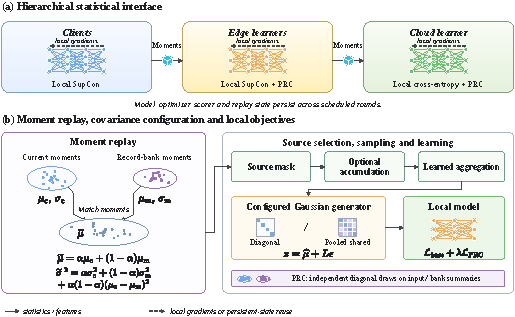
\includegraphics[width=\linewidth]{figures/method.drawio.pdf}
    \caption{Hierarchical training and upper-tier processing in \ehsfp{}. (a) Clients train on local examples; edge and cloud components train on synthesized features. Class-wise moments connect the tiers, with additional scatter for optional shared-covariance synthesis. (b) Moment replay, source masking, optional accumulation, and learned aggregation prepare the Gaussian training inputs. Classification supports diagonal or full shared covariance with diagonal fallback. PRC compares independent diagonal draws from input-side and memory summaries. Solid arrows denote statistics or feature flow. Dashed arrows denote local gradients or persistent-state reuse. The replay equation omits numerical jitter. Separate model synchronization and the ISIC-2018 supervised decoder stage are omitted.}
    \label{fig:hsfp_framework}
\end{figure*}

\subsection{Prototype Memory and Moment Replay}
\label{sec:memory}

The client--edge bank stores summaries from clients, and the edge--cloud bank stores summaries from edges. Each record contains class moments, support count, source identifier, generation round, age, and retrieval score. New summaries enter the bank before replay and keep their generation timestamps. Capacity enforcement favors more recent records. If a per-class cap applies, exceeding it removes a record of the highest age for that class. By default, each bank holds up to 500 records with a 20-round retention limit and no separate per-class cap.

For each class, the implementation retrieves up to $K_{\mathrm{mem}}=5$ records by default to form the memory moments $(\pmu_{\mathrm m}^{(j)},\psigma_{\mathrm m}^{(j)})$. It aggregates them with the total-variance rule in~\eqref{eq:agg_mean_var}, using normalized retrieval scores or uniform weights if their sum is below $\zeta$. The implemented retrieval scores stay at one and are separate from the learned aggregation scores. Record order breaks ties, and retrieval may include summaries that arrived in the current round.

When replay is enabled and $\alpha<1$, each existing source $\ell$ combines its current moments with the memory moments for each class represented in both sets. The combined moments are
\begin{equation}
\begin{split}
 \widetilde{\pmu}_{\ell}^{(j)}
 &=\alpha\pmu_{\mathrm c,\ell}^{(j)}
 +(1-\alpha)\pmu_{\mathrm m}^{(j)},\\
 (\widetilde{\psigma}_{\ell}^{(j)})^2
 &=\alpha(\psigma_{\mathrm c,\ell}^{(j)})^2
 +(1-\alpha)(\psigma_{\mathrm m}^{(j)})^2\\
 &\quad+\alpha(1-\alpha)
 (\pmu_{\mathrm c,\ell}^{(j)}-\pmu_{\mathrm m}^{(j)})^2+\zeta .
\end{split}
\label{eq:memory_mixture}
\end{equation}
Squares are coordinate-wise. The mixing coefficient $\alpha\in[0,1]$ weights the current moments, with a default of $0.3$ and $\alpha=1$ bypassing replay. With replay active, a class represented on only one side uses that side's moments. Equation~\eqref{eq:memory_mixture} gives the mixture mean and coordinate-wise variance with added jitter $\zeta$, which we set to $\zeta=10^{-8}$ as a numerical safeguard. The generator samples from a single Gaussian with these moments. \reviewblue{Proposition~\ref{prop:replay_drift} bounds the drift that this mixing adds when the current moments are fresh.} Replay can add a class found only in memory to an existing source output. An empty packet collection gives replay no source output to augment. The controller ages records and removes expired ones at the end of the round, so a delayed arrival may be used before this step.

\subsection{Source Masking and Learned Aggregation}
\label{sec:reliability}
\label{sec:dropout}

After replay, the mask independently marks each source output for removal with probability $\dropoutp_{\mathrm{train}}$. If it marks every output in a nonempty collection, the learner restores one chosen uniformly at random. A single source is always retained, and an empty collection stays empty. This restoration step makes the final retention indicators generally dependent. \reviewblue{Proposition~\ref{prop:masking_coverage} gives the resulting class-loss probability in closed form.} A masked source can already have contributed to the record bank. The retained sources can still omit classes or yield too few synthetic features for a valid minibatch.

Optional edge accumulation combines the retained outputs into one effective source. For each class, it maintains a decayed support total $A_0$ and support-weighted sums $A_1$ and $A_2$ of first and second raw moments. With decay $\gamma$, the update is
\begin{equation}
 (A_0,A_1,A_2)\leftarrow
 \gamma(A_0,A_1,A_2)
 +\sum_{\ell}n_\ell
 \bigl(1,\pmu_\ell,\psigma_\ell^2+\pmu_\ell^2\bigr).
 \label{eq:accumulated_moments}
\end{equation}
Missing or zero support receives unit weight. The accumulator reconstructs the mean as $A_1/A_0$ and the coordinate-wise variance as $\max\{A_2/A_0-(A_1/A_0)^2,\zeta\}$. It rounds the effective counts for use as metadata. The same decay applies to available scatter statistics and their degrees of freedom. The edge sees one effective source after accumulation. Contributions decay without a hard age cutoff.

For class $j$, let $\mathcal S^{(j)}$ index the resulting sources. The scorer uses support, spread $s_\ell=\|\psigma_\ell^{(j)}\|_2$, age $a_\ell$, and distance $d_\ell$ from the arithmetic mean of the source means for that class. Its six inputs are normalized log support, normalized spread, normalized age, normalized distance, a constant one, and a second copy of normalized log support. The support feature is $\log(1+n_\ell)/\log(1+\max\{1,n_{\max}\})$, with missing support set to zero. The spread and distance denominators are their respective class maxima, each floored at $\zeta$. The age denominator is the class maximum age, floored at one. A $6$--$32$--$32$--$1$ ReLU network with sigmoid output produces the source scores $f_\phi(v_\ell^{(j)})$. The corresponding weights are
\begin{equation}
 \omega_\ell^{(j)}
 =\frac{f_\phi(v_\ell^{(j)})}
 {\max\{\sum_{q\in\mathcal S^{(j)}}f_\phi(v_q^{(j)}),\zeta\}} .
 \label{eq:reliability_weight}
\end{equation}
The weights sum to one when the score sum is at least $\zeta$. When the floor is active, their sum is below one. The implementation uses these safeguarded weights in the class moment estimates
\begin{equation}
\begin{split}
 \widehat{\pmu}^{(j)}
 &=\sum_{\ell\in\mathcal S^{(j)}}\omega_\ell^{(j)}\pmu_\ell^{(j)},\\
 (\widehat{\psigma}^{(j)})^2
 &=\sum_{\ell\in\mathcal S^{(j)}}\omega_\ell^{(j)}
 \bigl[(\psigma_\ell^{(j)})^2
 +(\pmu_\ell^{(j)}-\widehat{\pmu}^{(j)})^2\bigr]+\zeta .
\end{split}
\label{eq:agg_mean_var}
\end{equation}
Count-weighted aggregation instead uses normalized support counts, with uniform weights when all counts are zero. The legacy uniform rule averages coordinate-wise variances without the between-source mean term. Comparisons with this rule therefore change both weighting and variance construction.

After round-end bank maintenance, the implementation trains the shared scorer using targets computed from record metadata. Each class in the client bank with at least two records contributes one mean-squared-error training step. The target averages $\min(n/100,1)$, $(1+s)^{-1}$, and $(1+a)^{-1}$, using $0.5$ for the support term when $n\le0$. The scorer defaults to Adam with learning rate $10^{-3}$ and weight decay $10^{-4}$. Its learned scores serve as proxies for source reliability. \reviewblue{Each of the three contributions is bounded in $[0,1]$. Their equal coefficients give support, compactness, and recency the same nominal scale, while 100 is a fixed support scale at which the count contribution saturates. These are implemented heuristic choices, not calibrated coefficients or consequences of the convergence analysis; the bootstrap target is not derived from downstream task loss and has no optimality guarantee. Proposition~\ref{prop:weighting_shift} shows that its effect on the synthetic mean is confined to classes whose sources disagree.}

\subsection{Gaussian Feature Synthesis}
\label{sec:lowrank}

Diagonal synthesis applies~\eqref{eq:prelim_synthesis} to the aggregated moments. Classification additionally supports a full covariance shared across classes. Each reporting source supplies within-class scatter
$S_\ell=\sum_i(x_{\ell i}-\pmu_\ell^{(y_{\ell i})})(x_{\ell i}-\pmu_\ell^{(y_{\ell i})})^\top$,
where $x_{\ell i}$ is a feature vector and $y_{\ell i}$ is its class label. The source also reports its sample count $N_\ell$ and represented-class count $C_\ell$. Pooling the source statistics gives
\begin{equation}
 \nu=\sum_\ell(N_\ell-C_\ell),\qquad
 \Sigma_0=\frac{\sum_\ell S_\ell}{\nu},\quad \nu>1.
 \label{eq:pooled_covariance}
\end{equation}
The instantaneous estimate is
$\Sigma=(1-\beta)\Sigma_0+\beta\operatorname{diag}(\Sigma_0)$,
where $\beta=\max\{0,1-\nu/(2d)\}$.
When accumulation is enabled, the covariance uses the ratio of accumulated scatter to the corresponding accumulated degrees of freedom.
\reviewblue{Shrinkage toward a diagonal covariance target is a standard stabilization strategy~\cite{schafer2005shrinkage}. Here the target is exactly $\operatorname{diag}(\Sigma_0)$, but the implemented coefficient $\beta=\max\{0,1-\nu/(2d)\}$ is a degrees-of-freedom heuristic rather than the data-estimated coefficient of~\cite{schafer2005shrinkage}. Remark~\ref{rem:scatter_pooling} notes that $\Sigma_0$ omits between-source variation of class means.}

For Cholesky factorization, the learner attempts
$\Sigma+\epsilon_{\mathrm{chol}}s_\Sigma I_d$,
where $s_\Sigma=\max\{\operatorname{tr}(\Sigma)/d,\zeta\}$ and the successive coefficients are $10^{-4},10^{-3},10^{-2},10^{-1}$. The first successful factor yields
\begin{equation}
 z^{(j)}=\widehat{\pmu}^{(j)}+L\epsilon,
 \qquad \epsilon\sim\mathcal N(0,I_d).
 \label{eq:lowrank_synthesis}
\end{equation}
The generator refreshes the covariance before drawing each training pool. A successful factorization uses $LL^\top$ for the main classification pool. The generator uses diagonal synthesis if the full covariance is missing or incompatible, or if all factorization attempts fail. Segmentation and PRC use diagonal synthesis.

\subsection{Local Objectives and Replay Consistency}
\label{sec:regularization}
\label{sec:prc}

Classification clients and edges use supervised contrastive loss~\cite{khosla2020supervised}. Each example supplies two independently transformed views whose outputs are pooled and $\ell_2$-normalized. Other views with the same label form the positive set, and every non-anchor view enters the denominator. Spatial feature maps use crop, flip, and blur transformations. Pooled edge features use additive noise and feature dropout. The client objective can also include a supervised loss. The cloud classification objective uses cross-entropy.

PRC compares the model outputs on pairs of features sampled independently from two class-conditional Gaussians. The first Gaussian uses the replayed source outputs. It averages their means uniformly and uses the root mean square of their standard deviations. The second Gaussian uses moments aggregated from all bank records with their stored scores. At the edge, the learner prepares the first set of moments before local masking and accumulation. At the cloud, it prepares them after masking. The two sets of moments can therefore use some of the same records. For the shared class set $\mathcal C$, let $C=|\mathcal C|>0$ and
$s=\min\{s_{\mathrm{req}},\max(1,\lfloor128/C\rfloor)\}$.
Using $s$ independent pairs from the two diagonal Gaussians for each shared class, the loss is
\begin{equation}
 \mathcal L_{\mathrm{PRC}}
 =\frac{1}{Csd_h}\sum_{j\in\mathcal C}\sum_{a=1}^{s}
 \|h(z_{\mathrm c,a}^{(j)})-h(z_{\mathrm m,a}^{(j)})\|_2^2 .
 \label{eq:prc_loss}
\end{equation}
Here $h$ returns pooled edge representations or cloud logits, and $d_h$ is its output dimension. The loss is zero when $C=0$. The summaries are detached from the computation graph, and gradients pass through both evaluations of $h$. The learner holds the summaries fixed during a phase and samples new pairs for each update that uses PRC. The implementation defaults are $s_{\mathrm{req}}=16$ and $\lambda_{\mathrm{prc}}=0.1$.

The independent draws determine how PRC acts on the outputs. For a fixed deterministic $h$, let $m_b^{(j)}$ and $V_b^{(j)}$ denote its output mean and covariance under side $b\in\{\mathrm c,\mathrm m\}$. Expanding the squared difference gives
\begin{equation}
\begin{split}
 \mathbb E\mathcal L_{\mathrm{PRC}}
 =\frac{1}{Cd_h}\sum_{j\in\mathcal C}
 \bigl(&\|m_{\mathrm c}^{(j)}-m_{\mathrm m}^{(j)}\|_2^2\\
 &+\operatorname{tr}V_{\mathrm c}^{(j)}
 +\operatorname{tr}V_{\mathrm m}^{(j)}\bigr).
\end{split}
\label{eq:prc_decomp}
\end{equation}
For this fixed output map, the expected penalty includes both the discrepancy between the output means and the output variation under each sampling law. \reviewblue{Consequently, $\mathbb E\mathcal L_{\mathrm{PRC}}$ is not minimized by matching the two output laws: even when they coincide, it equals $2(Cd_h)^{-1}\sum_j\operatorname{tr}V^{(j)}$, so PRC also contracts the output variance of $h$ on each class. This contraction may act as a class-compactness regularizer, but it also means that PRC is not a pure consistency penalty.}

The classification upper-tier objectives are
\begin{align}
 \mathcal L_e&=\mathcal L_{\mathrm{SupCon}}
 +\lambda_{\mathrm{prc}}\mathcal L_{\mathrm{PRC}},
 \label{eq:edge_loss}\\
 \mathcal L_g&=\mathcal L_{\mathrm{CE}}
 +\lambda_{\mathrm{prc}}\mathcal L_{\mathrm{PRC},g}.
 \label{eq:cloud_loss}
\end{align}
Source masking changes the synthetic inputs to the base objective. PRC provides the explicit output penalty. For ISIC-2018, a separate supervised stage trains the cloud decoder on image-specific features from frozen upstream modules and target masks using a Dice--focal loss.

\subsection{Processing and Cost}
\label{sec:processing_cost}

Algorithm~\ref{alg:ehsfp} separates preparation of the source summaries from local training. Each phase draws a labeled pool with $n_{\mathrm{syn}}$ examples per active class. The learner reuses this pool for $E$ shuffled epochs and discards incomplete final batches. With $J$ active classes and batch size $B$, the nominal budget is $E\lfloor Jn_{\mathrm{syn}}/B\rfloor$ updates before any execution truncation. The implementation defaults to $n_{\mathrm{syn}}=50$ and $E=10$ and allows each tier to override them. Without a full minibatch, the learner skips optimization. An edge can still extract output summaries from a nonempty pool. A separate draw configured for extraction adds no optimizer steps.

\begin{algorithm}[t]
\caption{Preparation and training at one prototype interface}
\label{alg:ehsfp}
\begin{enumerate}
 \item Insert received summaries into the interface bank, enforce capacity, and moment-mix existing source outputs.
 \item For each addressed learner:
 \begin{enumerate}
  \item Select assigned outputs; apply masking and optional edge accumulation, retaining PRC inputs at the tier-specific point in Section~\ref{sec:prc}.
  \item Aggregate moments, refresh covariance, and draw a labeled pool.
  \item Optimize the local objective within the execution budget; extract edge-output summaries when applicable and retain learning state.
 \end{enumerate}
\end{enumerate}
\end{algorithm}

At the end of each round, after the phases at both interfaces, the controller ages the records, removes expired ones, and trains the shared reliability network once. Model synchronization follows the separate schedules in Section~\ref{sec:formulation}.

For feature dimension $d$, a basic packet contains $2d+1$ scalars per class. Full covariance adds source-level scatter of size $O(d^2)$. The scatter traffic counter assigns $4d(d+1)/2$ bytes to a float32 upper triangle, compared with $4d^2$ bytes for dense storage. Factors require $O(d^2)$ storage, each draw costs $O(d^2)$, and factorization costs $O(d^3)$. The class moments in a bank of $R$ records require $O(Rd)$ storage. Metadata, model synchronization, and segmentation feature/mask transfers add traffic. The estimates describe tensor sizes before serialization and deployment.

\section{Convergence Analysis}
\label{sec:convergence}

We analyze one edge or cloud learner relative to a base objective induced by complete, fresh statistics. Prototype drift compares the actual and fresh-reference feature distributions within an episode. Reference variation describes how the fresh-reference objective changes across updates.

Consider SGD-type updates $\theta_{u+1}=\theta_u-\eta g_u$ for $u=0,\ldots,T-1$, where $u$ counts valid optimizer updates. Packet ages still use logical rounds. Let $e(u)$ denote the episode that supplies update $u$, and write $Q_u=Q_{e(u)}$. We use the same convention for the reference distribution, active classes, weights, and drift. Define the population batch objective by
\begin{equation}
 F_{u,Q}(\theta)=
 \mathbb E_{\mathcal B\sim\mathsf S_u(Q)}
 [\ell_{\mathrm{base}}(\theta;\mathcal B)],
 \label{eq:tier_objective}
\end{equation}
where $\mathsf S_u$ constructs minibatches using the episode's active classes, class weights, and augmentation rule. The base loss $\ell_{\mathrm{base}}$ can be a supervised contrastive loss or a task loss. Write $F_u=F_{u,Q_u}$ for the objective under the actual feature distribution and $F_{*,u}=F_{u,Q_{*,u}}$ for its fresh-reference counterpart. Both use the same active classes and sampling rule. The drift $\drift_u$ in~\eqref{eq:prototype_drift} compares the two feature distributions using the covariances of their samplers.

\subsection{Assumptions}

Let $\mathcal F_u$ denote the information available before the stochastic draw for update $u$. It includes the current parameters, episode and synthesis state, generated pool, reference statistics, and preceding history.

\begin{assumption}[Reference regularity]
\label{asm:smooth}
Each $F_{*,u}$ is $L$-smooth and bounded below by a common $F_{\inf}$.
\end{assumption}

\begin{assumption}[Conditional update model]
\label{asm:variance}
The update direction admits the decomposition
\begin{equation}
 g_u=\nabla F_u(\theta_u)
 +b_u^{\mathrm{sys}}+b_u^{\mathrm{reg}}+\xi_u,
 \label{eq:gradient_model}
\end{equation}
where the biases are $\mathcal F_u$-measurable,
$\mathbb E[\xi_u\mid\mathcal F_u]=0$, and
$\mathbb E[\|\xi_u\|_2^2\mid\mathcal F_u]\le\sigma_g^2$.
The term $b_u^{\mathrm{reg}}$ is the conditional mean contribution from PRC, including its coefficient. The term $b_u^{\mathrm{sys}}$ captures additional conditional mean error relative to the population objective under $Q_u$, such as bias from reusing a finite pool or sampling from shuffled batches. The term $\xi_u$ accounts for the remaining stochastic variation.
\end{assumption}
Periodic model synchronization between rounds is covered whenever its parameter perturbations satisfy this update decomposition and the error bounds below.

\begin{assumption}[Distribution-sensitive gradients]
\label{asm:drift}
With active classes, weights, and batch construction held fixed,
\begin{equation}
\begin{split}
 &\|\nabla F_{u,Q}(\theta)-\nabla F_{u,Q'}(\theta)\|_2\\
 &\quad\le L_z\Bigl(
 \sum_{j\in\mathcal J_u}\pi_u^{(j)}
 W_2^2(Q^{(j)},Q'^{(j)})\Bigr)^{1/2}.
\end{split}
\label{eq:gradient_distribution_sensitivity}
\end{equation}
\end{assumption}

If the batch sampler admits a class-wise coupling with shared labels and augmentation, a batch parameter gradient that is uniformly $K_b$-Lipschitz in the joint vector of $b$ features gives $L_z=K_b\sqrt b$ for expected class proportions $\pi_u^{(j)}$. For the implemented batch-averaged supervised contrastive loss, $K_b=O(b^{-1/2})$ under the sufficient conditions in Appendix~\ref{supp:supcon_sensitivity}: a fixed positive temperature, independent per-view embeddings, normalized embeddings with bounded derivatives, and uniformly bounded first and second network derivatives. The all-pairs coupling does not change this scaling because each softmax weight is $O(1/b)$ under bounded logits. These conditions keep $L_z=O(1)$, but they do not cover arbitrary batch-dependent layers (such as active BatchNorm layers that couple views across a minibatch); Assumption~\ref{asm:drift} therefore remains explicit rather than being inferred from the loss alone.

\begin{assumption}[Additional mean error]
\label{asm:het_agg}
For nonnegative constants $H_{\mathrm{het}},H_{\mathrm{agg}}$,
$\mathbb E\|b_u^{\mathrm{sys}}\|_2^2
\le2(H_{\mathrm{het}}+H_{\mathrm{agg}})$.
This bound excludes effects already represented by $Q_u$.
\end{assumption}

\begin{assumption}[Reference variation]
\label{asm:slow}
The reference objectives satisfy the variation budget
\begin{equation}
 \mathbb E\sum_{u=1}^{T-1}\sup_\theta
 |F_{*,u}(\theta)-F_{*,u-1}(\theta)|\le V_T .
 \label{eq:reference_variation}
\end{equation}
This budget includes changes in lower-tier representations, synthesis state, active classes, weights, and sampling rules.
\end{assumption}

\subsection{Stationarity Bound}

The bound evaluates the gradients of the fresh-reference base objectives at the parameters visited by the learner. It separates prototype drift, additional mean update errors, and PRC contributions.

\begin{theorem}[Tier-wise stationarity]
\label{thm:convergence}
Under Assumptions~\ref{asm:smooth}--\ref{asm:slow}, let
$T\ge1$ and $\eta=\eta_0/\sqrt T\le1/L$, with $\eta_0>0$.
Define the finite quantities
$\Delta_F=\mathbb E F_{*,0}(\theta_0)-F_{\inf}$,
$\bar D_T=T^{-1}\sum_u\mathbb E[\drift_u]$, and
$\bar R_T=T^{-1}\sum_u\mathbb E\|b_u^{\mathrm{reg}}\|_2^2$,
where all sums run from $0$ to $T-1$. Then
\begin{equation}
\begin{split}
 \frac1T\sum_{u=0}^{T-1}
 \mathbb E\|\nabla F_{*,u}(\theta_u)\|_2^2
 \le{}&\frac{2(\Delta_F+V_T)}{\eta_0\sqrt T}+\frac{L\eta_0\sigma_g^2}{\sqrt T}
 +3L_z^2\bar D_T\\
 &+6(H_{\mathrm{het}}+H_{\mathrm{agg}})
 +3\bar R_T .
\end{split}
\label{eq:main_bound}
\end{equation}
Packet availability may be dependent.
\end{theorem}

\begin{proof}
\iffalse
First, write the update as a reference gradient plus bias and noise. Set $a_u=\nabla F_{*,u}(\theta_u)$ and
$b_u=\nabla F_u(\theta_u)-a_u+
b_u^{\mathrm{sys}}+b_u^{\mathrm{reg}}$,
so that $g_u=a_u+b_u+\xi_u$. Smoothness and conditional zero-mean noise give
\begin{equation}
\begin{split}
 \mathbb E_uF_{*,u}(\theta_{u+1})
 \le{}&F_{*,u}(\theta_u)
 -\eta\langle a_u,a_u+b_u\rangle\\
 &+\frac{L\eta^2}{2}
 \bigl(\|a_u+b_u\|_2^2+\sigma_g^2\bigr),
\end{split}
\label{eq:conditional_descent}
\end{equation}
where $\mathbb E_u$ denotes conditioning on $\mathcal F_u$.
Using
$-2\langle a,a+b\rangle=-\|a\|_2^2-\|a+b\|_2^2+\|b\|_2^2$
and $L\eta\le1$ yields
\begin{equation}
\begin{split}
 \mathbb E_uF_{*,u}(\theta_{u+1})
 \le{}&F_{*,u}(\theta_u)-\frac{\eta}{2}\|a_u\|_2^2\\
 &+\frac{\eta}{2}\|b_u\|_2^2
 +\frac{L\eta^2}{2}\sigma_g^2.
\end{split}
\label{eq:biased_descent}
\end{equation}

Next, the three-term squared-norm inequality and Assumptions~\ref{asm:drift} and~\ref{asm:het_agg} imply
\begin{equation}
\begin{split}
 \mathbb E\|b_u\|_2^2
 \le{}&3L_z^2\mathbb E[\drift_u]
 +6(H_{\mathrm{het}}+H_{\mathrm{agg}})+3\mathbb E\|b_u^{\mathrm{reg}}\|_2^2 .
\end{split}
\label{eq:total_bias_bound}
\end{equation}
This step requires no independence among the bias components.

Finally, account for changes in the reference objective through the identity
\begin{equation}
\begin{split}
 &\sum_{u=0}^{T-1}
 [F_{*,u}(\theta_u)-F_{*,u}(\theta_{u+1})]=F_{*,0}(\theta_0)-F_{*,T-1}(\theta_T)\\
 &\quad+\sum_{u=1}^{T-1}
 [F_{*,u}(\theta_u)-F_{*,u-1}(\theta_u)].
\end{split}
\label{eq:changing_reference_telescope}
\end{equation}
The expected right-hand side is at most $\Delta_F+V_T$ by the common lower bound and Assumption~\ref{asm:slow}. Summing~\eqref{eq:biased_descent}, taking expectations, and dividing by $\eta T/2$ gives
\begin{equation}
\begin{split}
 \frac1T\sum_{u=0}^{T-1}\mathbb E\|a_u\|_2^2
 \le{}&\frac{2(\Delta_F+V_T)}{\eta T}
 +L\eta\sigma_g^2\\
 &+\frac1T\sum_{u=0}^{T-1}\mathbb E\|b_u\|_2^2 .
\end{split}
\label{eq:average_descent}
\end{equation}
Substituting~\eqref{eq:total_bias_bound} and $\eta=\eta_0/\sqrt T$ proves~\eqref{eq:main_bound}.
\fi
The detailed descent and changing-reference argument is given in Appendix~\ref{supp:analysis}.
\end{proof}

\begin{corollary}[Fresh-prototype limit]
\label{cor:small_perturb}
Under Theorem~\ref{thm:convergence}, if
$\bar D_T=\bar R_T=H_{\mathrm{het}}=H_{\mathrm{agg}}=0$
and $V_T=O(1)$, the average squared reference-gradient norm is $O(T^{-1/2})$.
\end{corollary}
\begin{proof}
Only the first two terms of~\eqref{eq:main_bound} remain.
\end{proof}

\begin{remark}[Controlling the drift residual]
\label{rem:drift_residual}
The drift residual $3L_z^2\bar D_T$ links the bound to the mechanisms of Section~\ref{sec:formulation}. With fresh current packets, Proposition~\ref{prop:replay_drift} makes the replay contribution vanish linearly as $\alpha\to1$. Proposition~\ref{prop:masking_coverage} shows that masking enters mainly through coverage when classes are held by few sources, and Lemma~\ref{prop:drift_decomp} below makes the age contribution quadratic in the maximum contribution age $A$. The residual does not include the gaps $\varepsilon_{\mathrm{ref}}$ and $\varepsilon_{\mathrm{rep}}$ in~\eqref{eq:surrogate_hierarchy}, because the reference objective already incorporates them.
\end{remark}

The optimization and noise terms in~\eqref{eq:main_bound} scale as $O((1+V_T)/\sqrt T)$ and reduce to $O(T^{-1/2})$ when $V_T=O(1)$. For the right-hand side to vanish, the reference variation must satisfy $V_T=o(\sqrt T)$ and the residual terms for drift, mean update error, and PRC must also vanish. Because Theorem~\ref{thm:convergence} evaluates gradients conditioned on the represented classes $\mathcal J_u$, replay, masking, and PRC appear in~\eqref{eq:main_bound} solely through their within-$\mathcal J_u$ drift and regularization residuals ($3L_z^2\bar D_T$ and $3\bar R_T$); their stabilizing benefits---preserving class coverage $\kappa_u$ against missing classes $j\notin\mathcal J_u$ and smoothing cross-round reference jumps $V_T$---operate outside this fixed-$\mathcal J_u$ residual decomposition. Finally, the constant step size $\eta=\eta_0/\sqrt T$ uses a known horizon $T$ for algebraic simplicity (an anytime schedule $\eta_u=\eta_0/\sqrt{u+1}$ yields the analogous $O((1+V_T+\log T)/\sqrt T)$ scaling; see Section~\ref{sec:discussion} for the relation to the Adam experiments).

\subsection{Conditional Age Decomposition}

To relate drift to prototype age, we compare each synthetic distribution with one built by refreshing the moments of its contributing sources. This comparison requires conditions on how source statistics change over time and how these changes affect synthesis. We represent a Gaussian by its mean and positive semidefinite covariance square root $(\mu,\Sigma^{1/2})$. The norm for such pairs is $\|(v,B)\|_\oplus^2=\|v\|_2^2+\|B\|_F^2$.

\begin{assumption}[Contribution ages and pipeline sensitivity]
\label{asm:staleness}
Every underlying statistic contributing to synthesis, including replayed and accumulated contributions, has age at most
$A=\stale_{\max}+A_{\mathcal M}$ logical rounds (accounting for maximum arrival staleness $\stale_{\max}$ plus bank retention $A_{\mathcal M}$).
For each source, consecutive-round mean/covariance-square-root pairs differ by at most $\delta$ in $\|\cdot\|_\oplus$.
Holding source coverage, support counts, replay and reconstruction coefficients, realized aggregation weights, and synthesis hyperparameters fixed, perturbing every contributing source pair by at most $\epsilon$ changes each final generated pair by at most $L_{\mathrm{agg}}\epsilon$. This sensitivity condition includes covariance estimation, numerical regularization, and fallback.
\end{assumption}

Let $\widetilde Q_u^{(j)}$ denote the intermediate feature law obtained by refreshing the contributing moments while keeping the other quantities in Assumption~\ref{asm:staleness} fixed. Its remaining discrepancy from the complete fresh reference is
\begin{equation}
 \varepsilon_{\mathrm{pipe},u}
 =\sum_{j\in\mathcal J_u}\pi_u^{(j)}
 W_2^2(\widetilde Q_u^{(j)},Q_{*,u}^{(j)}).
 \label{eq:coverage_error}
\end{equation}
The law retains the episode's source coverage and other fixed quantities. The fresh reference uses complete statistics and recomputes its input-dependent synthesis quantities. The residual compares these laws over the represented classes.

\begin{lemma}[Age-dependent drift]
\label{prop:drift_decomp}
Under Assumption~\ref{asm:staleness},
\begin{equation}
 \mathbb E[\drift_u]\le
 2L_{\mathrm{agg}}^2A^2\delta^2
 +2\mathbb E[\varepsilon_{\mathrm{pipe},u}].
 \label{eq:drift_bound}
\end{equation}
\end{lemma}
\begin{proof}
\iffalse
For Gaussian laws with pairs $(\mu,B)$ and $(\mu',B')$, coupling through the same $\epsilon\sim\mathcal N(0,I_d)$ gives
$W_2^2(G,G')\le\mathbb E\|(\mu-\mu')+(B-B')\epsilon\|_2^2
=\|(\mu-\mu',B-B')\|_\oplus^2$.
Telescoping source motion over at most $A$ rounds and applying pipeline sensitivity therefore yields
$W_2^2(Q_u^{(j)},\widetilde Q_u^{(j)})
\le L_{\mathrm{agg}}^2A^2\delta^2$.
The squared triangle inequality bounds each class drift by
$2W_2^2(Q_u^{(j)},\widetilde Q_u^{(j)})
+2W_2^2(\widetilde Q_u^{(j)},Q_{*,u}^{(j)})$.
Weighting over classes and taking expectations proves the result.
\fi
The Gaussian coupling and age-decomposition algebra are given in Appendix~\ref{supp:analysis}.
\end{proof}

An untruncated accumulator can retain contributions from expired records, so applying Lemma~\ref{prop:drift_decomp} requires a separate age bound for all contributing statistics and the sensitivity condition in Assumption~\ref{asm:staleness}. Theorem~\ref{thm:convergence} uses the realized drift directly and does not require this decomposition. The bound does not cover class coverage and update frequency.
\section{Experimental Evaluation}
\label{sec:experiments}

\subsection{Experimental Setup}

\noindent\textbf{Datasets.}~
We evaluate \ehsfp{} on CIFAR-10/100~\cite{krizhevsky2009learning}, HAM10000~\cite{tschandl2018ham10000}, and ImageNet-1K~\cite{5206848} for classification and on ISIC-2018~\cite{codella2019isic2018} for segmentation.

\noindent\textbf{Baselines.}~
\hsfp{}~\cite{tran2026h} is the closest prior method. \ehsfp{} extends its class-wise statistical interface to upper-tier learning from incomplete and delayed summaries. Tables~\ref{tab:main_classification} and~\ref{tab:sweep_200} reproduce historical baseline values from the \hsfp{} study~\cite{tran2026h}. These comparisons include \hsfp{}, FedAvg~\cite{mcmahan2017communication}, FedProx~\cite{li2020federated}, FedProto~\cite{tan2022fedproto}, HierFL~\cite{liu2020client,9488756}, SplitFed~\cite{thapa2022splitfed}, HeteroSFL~\cite{chen2025heterosfl}, FedGen~\cite{zhu2021data}, FedDF~\cite{lin2020ensemble}, and HSFL~\cite{quan2023hiersfl}.

\begin{table*}[t]
\centering
\footnotesize
\caption{\reviewblue{Classification accuracy and ISIC-2018 segmentation results (reported mean $\pm$ standard deviation). \ehsfp{} rows reproduce the manuscript's journal aggregates; resolved per-seed 200-round records were not recovered locally. All other rows are reproduced from~\cite{tran2026h} under its protocol (ten edges; 200 devices for ISIC-2018) and are not matched runs; differences are descriptive.}}
\label{tab:main_classification}
\begin{tabular}{@{}lccccccc@{}}
\toprule
& \multicolumn{4}{c}{Classification accuracy (\%) $\uparrow$}
& \multicolumn{3}{c}{ISIC-2018} \\
\cmidrule(lr){2-5}\cmidrule(lr){6-8}
Method & CIFAR-10 & CIFAR-100 & HAM10000 & ImageNet-1K
& IoU (\%) $\uparrow$ & Dice (\%) $\uparrow$ & Time (h) $\downarrow$ \\
\midrule

FedAvg
& 57.25 {\scriptsize $\pm$ 1.24}
& 48.85 {\scriptsize $\pm$ 1.40}
& 68.28 {\scriptsize $\pm$ 1.45}
& 23.1 {\scriptsize $\pm$ 1.4}
& 48.7 {\scriptsize $\pm$ 1.2}
& 64.2 {\scriptsize $\pm$ 1.5}
& 28.5 {\scriptsize $\pm$ 0.8} \\

FedProx
& 58.25 {\scriptsize $\pm$ 1.20}
& 52.75 {\scriptsize $\pm$ 1.25}
& 71.15 {\scriptsize $\pm$ 1.30}
& 24.1 {\scriptsize $\pm$ 1.3}
& \textemdash
& \textemdash
& \textemdash \\

FedProto
& 55.10 {\scriptsize $\pm$ 1.05}
& 46.50 {\scriptsize $\pm$ 1.15}
& 67.20 {\scriptsize $\pm$ 1.25}
& 25.2 {\scriptsize $\pm$ 1.2}
& \textemdash
& \textemdash
& \textemdash \\

HierFL
& 62.50 {\scriptsize $\pm$ 1.30}
& 30.15 {\scriptsize $\pm$ 1.45}
& 69.50 {\scriptsize $\pm$ 1.25}
& 24.5 {\scriptsize $\pm$ 1.2}
& 51.2 {\scriptsize $\pm$ 1.1}
& 66.3 {\scriptsize $\pm$ 1.3}
& 24.3 {\scriptsize $\pm$ 0.7} \\

SplitFed
& 61.85 {\scriptsize $\pm$ 1.25}
& 35.00 {\scriptsize $\pm$ 1.30}
& 65.78 {\scriptsize $\pm$ 1.35}
& 25.5 {\scriptsize $\pm$ 1.1}
& 53.8 {\scriptsize $\pm$ 0.9}
& 68.1 {\scriptsize $\pm$ 1.1}
& 72.4 {\scriptsize $\pm$ 1.6} \\

HeteroSFL
& 63.45 {\scriptsize $\pm$ 1.10}
& 41.50 {\scriptsize $\pm$ 1.25}
& 67.10 {\scriptsize $\pm$ 1.20}
& 26.3 {\scriptsize $\pm$ 0.8}
& 56.4 {\scriptsize $\pm$ 0.7}
& 70.5 {\scriptsize $\pm$ 0.8}
& 45.8 {\scriptsize $\pm$ 1.2} \\

FedGen
& 59.80 {\scriptsize $\pm$ 1.10}
& 51.20 {\scriptsize $\pm$ 1.25}
& 72.50 {\scriptsize $\pm$ 1.15}
& 26.8 {\scriptsize $\pm$ 1.0}
& \textemdash
& \textemdash
& \textemdash \\

FedDF
& 61.50 {\scriptsize $\pm$ 1.15}
& 53.10 {\scriptsize $\pm$ 1.20}
& 73.10 {\scriptsize $\pm$ 1.20}
& 25.9 {\scriptsize $\pm$ 1.1}
& \textemdash
& \textemdash
& \textemdash \\

HSFL (A)
& 51.35 {\scriptsize $\pm$ 1.10}
& 35.47 {\scriptsize $\pm$ 1.35}
& 68.82 {\scriptsize $\pm$ 1.25}
& 24.6 {\scriptsize $\pm$ 0.9}
& 62.1 {\scriptsize $\pm$ 0.8}
& 74.8 {\scriptsize $\pm$ 0.9}
& 14.5 {\scriptsize $\pm$ 0.5} \\

H-SFP (A)
& 67.44 {\scriptsize $\pm$ 0.85}
& 55.10 {\scriptsize $\pm$ 0.95}
& 80.86 {\scriptsize $\pm$ 0.75}
& 27.9 {\scriptsize $\pm$ 0.3}
& 68.3 {\scriptsize $\pm$ 0.5}
& 79.5 {\scriptsize $\pm$ 0.4}
& 6.8 {\scriptsize $\pm$ 0.2} \\

\midrule


E-HSFP
& 68.13 {\scriptsize $\pm$ 0.81}
& 56.07 {\scriptsize $\pm$ 0.89}
& 81.27 {\scriptsize $\pm$ 0.71}
& 29.37 {\scriptsize $\pm$ 0.28}
& 69.12 {\scriptsize $\pm$ 0.46}
& 80.23 {\scriptsize $\pm$ 0.37}
& 6.67 {\scriptsize $\pm$ 0.19} \\

\bottomrule
\end{tabular}
\end{table*}

\noindent\textbf{\ehsfp{} protocol.}~
The manuscript reports each \ehsfp{} configuration as a 200-round, five-run experiment on a single NVIDIA RTX A6000 GPU with 48\,GB of memory. Unless otherwise specified, classification uses 200 clients assigned to five edge servers, with 10\% client participation per round. ISIC-2018 uses 50 clients. The reported settings include a batch size of 16, Adam with a learning rate and weight decay of $10^{-4}$ each, and a five-round warm-up. The implementation supports cosine decay after warm-up. Classification experiments use IID partitions and Dirichlet partitions with concentrations $0.70$ and $0.30$. \reviewblue{These statements describe the intended protocol, not a reconstruction from the retained archive: the locally retained matching records are 60-round development runs at $T_{\mathrm{temp}}=0.1$, and the retained CIFAR-100 \ehsfp{} $\mathrm{Dir}(0.30)$ and $\mathrm{Dir}(0.70)$ attempts contain only incomplete seed-0 jobs. Those records are excluded from the 200-round evidence.}

The reference condition uses a record retention limit of $A_{\mathcal M}=20$ logical rounds, a source-mask rate of $\dropoutp_{\mathrm{train}}=0.2$, and a contrastive temperature of $T_{\mathrm{temp}}=0.5$. The archived summaries identify this condition by the memory-control label $\memcap=10$. Section~\ref{sec:method} describes the implementation and its defaults.

\noindent\textbf{Scope of cross-study comparisons.}~
The ECCV experiments use ten edges for hierarchical methods and 200 devices for ISIC-2018~\cite{tran2026h}. The label (A) denotes the ECCV aggregation schedule with client--edge and edge--cloud intervals of 5 and 10 local epochs, respectively. The 50-client \ehsfp{} segmentation pipeline uses diagonal synthesis and trains a supervised decoder on target masks and features from frozen upstream models. Decoder schedules, update budgets, and timing boundaries could not be verified across studies. We therefore interpret score and runtime differences as descriptive comparisons across protocols. \reviewblue{In particular, the margins over \hsfp{} in Table~\ref{tab:main_classification} are small (0.4--1.5 percentage points) and come from different protocols, so they should not be read as evidence of improvement until matched runs are available.}

\noindent\textbf{Configuration provenance.}~
The archived summaries lack the resolved configuration and environment for each journal run, including exact model cuts and timing boundaries. The implementation meaning of $\memcap$ is also unresolved, including whether the label denotes a per-class record limit or controls statistics decay. Table~\ref{tab:ablation} retains the reported configuration labels. The stress levels, overrides, and exact generator for the full-synthesis row remain unspecified. \reviewblue{The current \texttt{full\_e\_hsfp} preset forces the serverless simulator on and is applied after individual configuration keys; a clean no-event reference must therefore enable the E-HSFP components explicitly without that preset. The preset's residual-generator flag is also inactive in the executed classification path, which initializes no residual generator; the implemented full-synthesis choice is instead \texttt{synthesis=shared\_cov}. The implemented drift logger does not evaluate the complete reference in~\eqref{eq:fresh_reference}. At an edge it uses only the freshly selected participating clients, weights classes by their recorded support, compares only shared classes, and computes the diagonal mean--standard-deviation Gaussian distance. It therefore omits unselected assigned sources and the shared-covariance sampler used by full synthesis. Its retained CSV reports shared and missing class counts but not the exact generated class set, task-class denominator, realized class weights, or sampler covariance. Logged drift is a participating-source diagonal diagnostic and is not reported as $\drift_t$.}

For the execution-event rows in Table~\ref{tab:robustness}, the records lack event probabilities, delay magnitudes, partial-execution fractions, and the composition of the combined event. Class coverage and the frequency of episodes without a valid minibatch are unavailable. These gaps limit reproducibility and attribution of differences to individual components. The execution-event results characterize simulated conditions, and measurements on a deployed system would be needed to assess operational costs.

\noindent\textbf{Metrics.}~
We report classification accuracy and macro-F1, segmentation IoU and Dice, training time, and relative convergence rounds (Conv.). To compute relative rounds, we smooth each run's validation accuracy with a three-round trailing average and find the first sequence of three consecutive smoothed values at or above 95\% of that run's best validation accuracy. We record the first round of that sequence. Differences between percentage scores are expressed in percentage points. The Adam experiments measure task performance and progress toward each run's own threshold. Section~\ref{sec:convergence} analyzes stationarity under a conditional SGD-type update model.

\subsection{Overall Performance}

Table~\ref{tab:main_classification} reports \ehsfp{} mean accuracies of 68.13\%, 56.07\%, 81.27\%, and 29.37\% on CIFAR-10, CIFAR-100, HAM10000, and ImageNet-1K, respectively. The 50-client ISIC-2018 pipeline reaches 69.12\% IoU and 80.23\% Dice, with a reported mean training time of 6.67 hours. Section~\ref{sec:processing_cost} distinguishes the basic prototype payload from the communication required by other stages.

\subsection{Robustness under Simulated Episodic Disruptions}
\begin{table}[t]
\centering
\footnotesize
\caption{Analyzing overall performance of \ehsfp{} on CIFAR-100 with IID setting under simulated episodic disruptions. Results are reported as the mean and standard deviation across 5 independent seeds.}
\label{tab:robustness}
\begin{tabular}{@{}lccc@{}}
\toprule
Condition & Acc. (\%) & F1 (\%) & Conv. \\
\midrule

E-HSFP
& 56.07 {\scriptsize $\pm$ 0.89}
& 57.01 {\scriptsize $\pm$ 0.97}
& 121.00 {\scriptsize $\pm$ 8.00} \\

\midrule
\multicolumn{4}{@{}l}{\textit{(a) Source masking, $\stale=0$}} \\

$\dropoutp_{\mathrm{train}}=0.00$
& 56.43 {\scriptsize $\pm$ 0.83}
& 57.39 {\scriptsize $\pm$ 0.89}
& 112.00 {\scriptsize $\pm$ 6.00} \\

$\dropoutp_{\mathrm{train}}=0.10$
& 56.28 {\scriptsize $\pm$ 0.86}
& 57.23 {\scriptsize $\pm$ 0.93}
& 116.00 {\scriptsize $\pm$ 7.00} \\

$\dropoutp_{\mathrm{train}}=0.30$
& 55.79 {\scriptsize $\pm$ 0.94}
& 56.68 {\scriptsize $\pm$ 1.03}
& 129.00 {\scriptsize $\pm$ 9.00} \\

$\dropoutp_{\mathrm{train}}=0.50$
& 55.13 {\scriptsize $\pm$ 1.07}
& 55.96 {\scriptsize $\pm$ 1.16}
& 148.00 {\scriptsize $\pm$ 11.00} \\

\midrule
\multicolumn{4}{@{}l}{\textit{(b) Delay, $\dropoutp_{\mathrm{train}}=0.20$}} \\

$\stale=1$
& 55.72 {\scriptsize $\pm$ 0.93}
& 56.59 {\scriptsize $\pm$ 1.01}
& 127.00 {\scriptsize $\pm$ 9.00} \\

$\stale=3$
& 55.18 {\scriptsize $\pm$ 1.03}
& 55.96 {\scriptsize $\pm$ 1.12}
& 138.00 {\scriptsize $\pm$ 10.00} \\

$\stale=5$
& 54.61 {\scriptsize $\pm$ 1.16}
& 55.34 {\scriptsize $\pm$ 1.24}
& 151.00 {\scriptsize $\pm$ 12.00} \\

$\stale=10$
& 53.47 {\scriptsize $\pm$ 1.37}
& 54.08 {\scriptsize $\pm$ 1.46}
& 176.00 {\scriptsize $\pm$ 14.00} \\

\midrule
\multicolumn{4}{@{}l}{\textit{(c) Added execution events}} \\

Function timeout
& 55.73 {\scriptsize $\pm$ 0.97}
& 56.62 {\scriptsize $\pm$ 1.06}
& 133.00 {\scriptsize $\pm$ 9.00} \\

Cold-start delay
& 55.86 {\scriptsize $\pm$ 0.93}
& 56.78 {\scriptsize $\pm$ 1.02}
& 128.00 {\scriptsize $\pm$ 9.00} \\

Partial edge execution
& 55.41 {\scriptsize $\pm$ 1.08}
& 56.23 {\scriptsize $\pm$ 1.17}
& 142.00 {\scriptsize $\pm$ 11.00} \\

Missing edge update
& 55.28 {\scriptsize $\pm$ 1.12}
& 56.07 {\scriptsize $\pm$ 1.21}
& 146.00 {\scriptsize $\pm$ 11.00} \\

Combined
& 54.13 {\scriptsize $\pm$ 1.31}
& 54.82 {\scriptsize $\pm$ 1.42}
& 169.00 {\scriptsize $\pm$ 13.00} \\

\bottomrule
\end{tabular}
\end{table}

\begin{table*}[t]
\centering
\caption{Reported configuration contrasts on CIFAR-100 IID (200 clients, 200 rounds; mean $\pm$ standard deviation over five runs). Accuracy and F1 are percentages. Conv.\ denotes relative rounds. The synthesis comparison reuses the PRC and full-synthesis summaries in (a). Labels $\memcap=10$ and $0$ reuse the full-synthesis and learned-weighting summaries, respectively.}
\label{tab:ablation}
\begin{tabular}{@{}l|ccccc@{}}
\toprule
Variant & Acc. (\%) & F1 (\%) & Conv.
& \shortstack{Acc.\ under\\source masking}
& \shortstack{Acc.\ under\\staleness} \\
\midrule
\multicolumn{6}{@{}l}{\textit{(a) Reported \ehsfp{} configurations}} \\

Episodic memory
& 55.02 {\scriptsize $\pm$ 0.97}
& 55.91 {\scriptsize $\pm$ 1.05}
& 130.00 {\scriptsize $\pm$ 10.00}
& 53.83 {\scriptsize $\pm$ 1.11}
& 52.38 {\scriptsize $\pm$ 1.33} \\

Source masking configuration
& 55.19 {\scriptsize $\pm$ 0.95}
& 56.08 {\scriptsize $\pm$ 1.03}
& 129.00 {\scriptsize $\pm$ 9.00}
& 54.37 {\scriptsize $\pm$ 1.09}
& 52.41 {\scriptsize $\pm$ 1.35} \\

Learned weighting configuration
& 55.36 {\scriptsize $\pm$ 0.93}
& 56.24 {\scriptsize $\pm$ 1.01}
& 127.00 {\scriptsize $\pm$ 9.00}
& 54.63 {\scriptsize $\pm$ 1.07}
& 52.89 {\scriptsize $\pm$ 1.31} \\

PRC configuration (diagonal)
& 55.43 {\scriptsize $\pm$ 0.97}
& 56.29 {\scriptsize $\pm$ 1.03}
& 125.00 {\scriptsize $\pm$ 9.00}
& 54.71 {\scriptsize $\pm$ 1.11}
& 53.07 {\scriptsize $\pm$ 1.39} \\

Reported full synthesis
& 56.07 {\scriptsize $\pm$ 0.89}
& 57.01 {\scriptsize $\pm$ 0.97}
& 121.00 {\scriptsize $\pm$ 8.00}
& 55.13 {\scriptsize $\pm$ 1.07}
& 53.47 {\scriptsize $\pm$ 1.37} \\

\midrule
\multicolumn{6}{@{}l}{\textit{(b) Aggregation rows labeled $\memcap=0$}} \\

Legacy uniform
& 55.17 {\scriptsize $\pm$ 1.01}
& 56.08 {\scriptsize $\pm$ 1.07}
& 132.00 {\scriptsize $\pm$ 10.00}
& 53.14 {\scriptsize $\pm$ 1.27}
& 51.43 {\scriptsize $\pm$ 1.51} \\

Sample-count weighted
& 55.34 {\scriptsize $\pm$ 0.99}
& 56.21 {\scriptsize $\pm$ 1.05}
& 130.00 {\scriptsize $\pm$ 9.00}
& 53.47 {\scriptsize $\pm$ 1.23}
& 51.71 {\scriptsize $\pm$ 1.47} \\

Learned weighting
& 55.68 {\scriptsize $\pm$ 0.97}
& 56.57 {\scriptsize $\pm$ 1.03}
& 126.00 {\scriptsize $\pm$ 9.00}
& 53.78 {\scriptsize $\pm$ 1.19}
& 51.86 {\scriptsize $\pm$ 1.43} \\

\midrule
\multicolumn{6}{@{}l}{\textit{(c) Additional memory-control labels}} \\

$\memcap=1$
& 55.81 {\scriptsize $\pm$ 0.95}
& 56.72 {\scriptsize $\pm$ 1.01}
& 124.00 {\scriptsize $\pm$ 9.00}
& 54.21 {\scriptsize $\pm$ 1.13}
& 52.37 {\scriptsize $\pm$ 1.41} \\

$\memcap=5$
& 55.98 {\scriptsize $\pm$ 0.91}
& 56.93 {\scriptsize $\pm$ 0.99}
& 122.00 {\scriptsize $\pm$ 8.00}
& 54.87 {\scriptsize $\pm$ 1.09}
& 53.12 {\scriptsize $\pm$ 1.39} \\

$\memcap=20$
& 56.02 {\scriptsize $\pm$ 0.93}
& 56.94 {\scriptsize $\pm$ 1.01}
& 123.00 {\scriptsize $\pm$ 9.00}
& 55.27 {\scriptsize $\pm$ 1.03}
& 53.69 {\scriptsize $\pm$ 1.29} \\

\bottomrule
\end{tabular}
\end{table*}

\begin{table*}[t]
\centering
\footnotesize
\caption{Architecture, client-count, and temperature sensitivity (\%, reported mean $\pm$ standard deviation). The intended protocol uses 200 rounds, five runs, 200 clients, and $T_{\mathrm{temp}}=0.5$ unless varied; resolved per-seed 200-round \ehsfp{} records were not recovered. The $T_{\mathrm{temp}}=0.5$ H-SFP cells are reproduced from the published ECCV temperature table~\cite{tran2026h}. \reviewpurple{The \ehsfp{} IID entries remain as reported manuscript aggregates because they agree with Figure~\ref{fig:partition_accuracy}; the three $\mathrm{Dir}(0.7)$ entries are unavailable because the table and figure disagree and neither source has recoverable five-seed provenance.} Client-count sweeps use IID data. R50 denotes ResNet-50, and HAM denotes HAM10000.}
\label{tab:sweep_200}
\setlength{\tabcolsep}{2pt}
\begin{minipage}[t]{0.42\textwidth}
\centering
\begin{tabular}{@{}l|cc@{}}
\toprule
Setting & H-SFP  & E-HSFP \\
\midrule
\multicolumn{3}{@{}l}{\textit{(a) Additional architecture/partition settings}} \\

HAM, VGG16, IID
& 78.45 {\scriptsize $\pm$ 0.80}
& 79.03 {\scriptsize $\pm$ 0.77} \\

ImageNet, VGG16, IID
& 25.3 {\scriptsize $\pm$ 0.4}
& 26.89 {\scriptsize $\pm$ 0.41} \\

ImageNet, R50, $\mathrm{Dir}(0.7)$
& 22.4 {\scriptsize $\pm$ 0.6}
& 24.03 {\scriptsize $\pm$ 0.57} \\

\midrule
\multicolumn{3}{@{}l}{\textit{(b) ImageNet-1K clients, IID}} \\

20
& 64.8 {\scriptsize $\pm$ 0.2}
& 65.63 {\scriptsize $\pm$ 0.21} \\

50
& 51.5 {\scriptsize $\pm$ 0.3}
& 52.61 {\scriptsize $\pm$ 0.31} \\

100
& 38.4 {\scriptsize $\pm$ 0.3}
& 39.72 {\scriptsize $\pm$ 0.29} \\

\midrule
\multicolumn{3}{@{}l}{\textit{(c) CIFAR-100 clients, IID}} \\

20
& 67.80 {\scriptsize $\pm$ 0.60}
& 68.49 {\scriptsize $\pm$ 0.57} \\

50
& 64.50 {\scriptsize $\pm$ 0.75}
& 65.31 {\scriptsize $\pm$ 0.71} \\

100
& 60.20 {\scriptsize $\pm$ 0.85}
& 61.08 {\scriptsize $\pm$ 0.79} \\

500
& \reviewpurple{\textemdash}
& 49.07 {\scriptsize $\pm$ 1.13} \\

\bottomrule
\end{tabular}
\end{minipage}\hfill
\begin{minipage}[t]{0.56\textwidth}
\centering
\resizebox{\linewidth}{!}{%
\begin{tabular}{@{}llccccc@{}}
\toprule
& & \multicolumn{5}{c}{\textit{(d) Temperature $T_{\mathrm{temp}}$}} \\
\cmidrule(lr){3-7}
Setting & Method & $0.20$ & $0.50$ & $1.00$ & $1.50$ & $2.00$ \\
\midrule

CIFAR-10, IID & H-SFP
& 55.30 {\scriptsize $\pm$ 1.15}
& 67.44 {\scriptsize $\pm$ 0.85}
& 63.15 {\scriptsize $\pm$ 0.95}
& 60.03 {\scriptsize $\pm$ 1.05}
& 56.38 {\scriptsize $\pm$ 1.10} \\

 & E-HSFP
& 56.42 {\scriptsize $\pm$ 1.09}
& 68.13 {\scriptsize $\pm$ 0.81}
& 64.07 {\scriptsize $\pm$ 0.91}
& 61.02 {\scriptsize $\pm$ 0.97}
& 57.51 {\scriptsize $\pm$ 1.03} \\

\addlinespace[2pt]

CIFAR-10, $\mathrm{Dir}(0.7)$ & H-SFP
& 36.20 {\scriptsize $\pm$ 1.35}
& 48.85 {\scriptsize $\pm$ 1.10}
& 43.10 {\scriptsize $\pm$ 1.20}
& 41.50 {\scriptsize $\pm$ 1.25}
& 38.40 {\scriptsize $\pm$ 1.30} \\

 & E-HSFP
& 37.64 {\scriptsize $\pm$ 1.29}
& 49.31 {\scriptsize $\pm$ 1.22}
& 44.43 {\scriptsize $\pm$ 1.13}
& 42.91 {\scriptsize $\pm$ 1.19}
& 39.89 {\scriptsize $\pm$ 1.23} \\

\addlinespace[2pt]

CIFAR-100, IID & H-SFP
& 48.15 {\scriptsize $\pm$ 1.20}
& 55.10 {\scriptsize $\pm$ 0.95}
& 52.88 {\scriptsize $\pm$ 1.05}
& 51.10 {\scriptsize $\pm$ 1.10}
& 48.65 {\scriptsize $\pm$ 1.15} \\

 & E-HSFP
& 49.31 {\scriptsize $\pm$ 1.13}
& 56.07 {\scriptsize $\pm$ 0.89}
& 53.97 {\scriptsize $\pm$ 0.99}
& 52.28 {\scriptsize $\pm$ 1.03}
& 49.87 {\scriptsize $\pm$ 1.09} \\

\addlinespace[2pt]

CIFAR-100, $\mathrm{Dir}(0.7)$ & H-SFP
& 6.20 {\scriptsize $\pm$ 0.95}
& 10.48 {\scriptsize $\pm$ 0.85}
& 8.50 {\scriptsize $\pm$ 0.90}
& 7.20 {\scriptsize $\pm$ 0.95}
& 6.05 {\scriptsize $\pm$ 1.00} \\

 & E-HSFP
& 8.16 {\scriptsize $\pm$ 0.97}
& 11.02 {\scriptsize $\pm$ 0.83}
& 10.43 {\scriptsize $\pm$ 0.93}
& 9.17 {\scriptsize $\pm$ 0.97}
& 8.09 {\scriptsize $\pm$ 1.01} \\

\addlinespace[2pt]

HAM, IID & H-SFP
& 71.42 {\scriptsize $\pm$ 1.10}
& 80.86 {\scriptsize $\pm$ 0.75}
& 77.40 {\scriptsize $\pm$ 0.90}
& 75.85 {\scriptsize $\pm$ 0.95}
& 72.12 {\scriptsize $\pm$ 1.05} \\

 & E-HSFP
& 72.18 {\scriptsize $\pm$ 1.03}
& 81.27 {\scriptsize $\pm$ 0.71}
& 78.02 {\scriptsize $\pm$ 0.83}
& 76.57 {\scriptsize $\pm$ 0.89}
& 72.93 {\scriptsize $\pm$ 0.99} \\

\addlinespace[2pt]

HAM, $\mathrm{Dir}(0.7)$ & H-SFP
& 30.55 {\scriptsize $\pm$ 1.25}
& 37.50 {\scriptsize $\pm$ 1.05}
& 34.70 {\scriptsize $\pm$ 1.15}
& 33.10 {\scriptsize $\pm$ 1.20}
& 30.45 {\scriptsize $\pm$ 1.25} \\

 & E-HSFP
& 32.08 {\scriptsize $\pm$ 1.19}
& 38.12 {\scriptsize $\pm$ 1.03}
& 36.18 {\scriptsize $\pm$ 1.09}
& 34.63 {\scriptsize $\pm$ 1.13}
& 32.03 {\scriptsize $\pm$ 1.19} \\

\bottomrule
\end{tabular}
}
\end{minipage}
\end{table*}
Table~\ref{tab:robustness} reports \ehsfp{} performance under simulated input and execution disruptions on IID CIFAR-100. The first row gives the reference setting with source-mask rate $\dropoutp_{\mathrm{train}}=0.2$ and zero injected delay, before additional execution events. The mask sweep holds the maximum injected delay at $\stale=0$. The delay sweep holds the source-mask rate at $\dropoutp_{\mathrm{train}}=0.2$ and samples integer delays uniformly from $\{0,\ldots,\stale\}$. The training mask acts on source outputs after memory insertion and replay and restores one output if all are removed. \reviewblue{Note that the mask sweep varies the training-time mask, which is part of the method, rather than an external disruption applied at fixed training settings. The sweep therefore measures the cost of the regularizer, not robustness to lost packets.} Section~\ref{sec:dropout} describes the mask, and Section~\ref{sec:formulation} defines the independent packet-delivery model.

As the mask rate rises from $0$ to $0.5$, mean accuracy falls by 1.30 percentage points and the mean relative-round count rises from 112 to 148. As the maximum delay rises from $0$ to $10$ rounds, mean accuracy falls by 2.60 percentage points and the count rises from 121 to 176. The individual execution-event conditions yield mean accuracies 0.21--0.79 percentage points below the reference. The combined condition yields 54.13\% accuracy, 54.82\% macro-F1, and a mean relative-round count of 169. \reviewblue{Within both sweeps, the difference between adjacent settings is smaller than the corresponding five-run standard deviations, and no significance tests are reported. The setting $p_{\mathrm{train}}=0$ has the highest mean accuracy and the fewest relative rounds, so these simulations do not show a benefit of the default mask rate 0.2. Proposition~\ref{prop:masking_coverage} offers one explanation that remains to be tested: under IID partitions, most classes are held by every source, so masking rarely removes a class and mainly perturbs the aggregated moments.} \reviewred{[Evidence gap: the retained diagnostics do not record the generated active-class set and task-class denominator needed for $\kappa_t$, nor all-assigned fresh packets, realized class weights, and the actual shared-covariance sampler needed for $\drift_t$. The existing participating-source diagonal diagnostic is not the quantity in~\eqref{eq:prototype_drift}; upgraded diagnostics and matched 200-round sweep runs are required.]}

\subsection{Statistical Heterogeneity and Relative Convergence}

\begin{figure}[t]
    \centering
    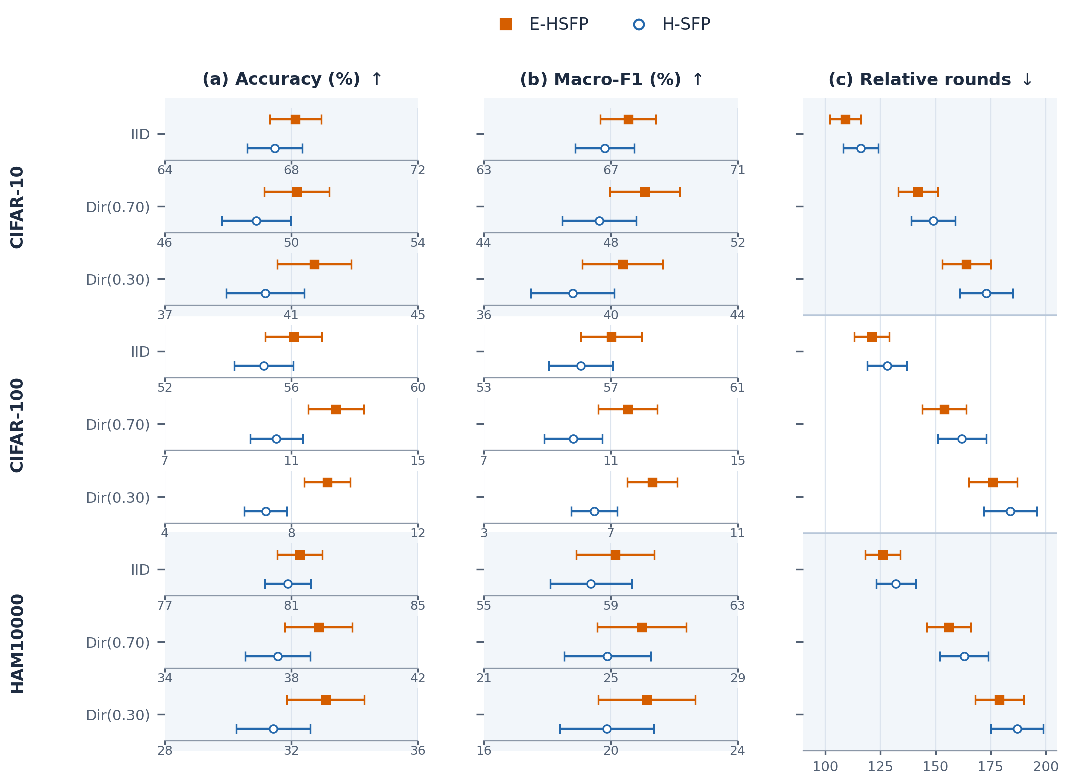
\includegraphics[width=\linewidth]{figures/fig_partition_comparison.pdf}
    \caption{Partition sensitivity reported as mean $\pm$ standard deviation for H-SFP and E-HSFP across 3 datasets. \reviewpurple{The plotting source describes these values as five-seed aggregates, but resolved per-seed 200-round records were not recovered locally.} Relative rounds use the run-specific validation criterion in Section~\ref{sec:experiments}.}
    \label{fig:partition_accuracy}
\end{figure}
Figure~\ref{fig:partition_accuracy} compares classification performance and training progress across nine dataset--partition settings. For \ehsfp{}, mean accuracy falls from 68.13\%, 56.07\%, and 81.27\% under IID to 41.73\%, 9.13\%, and 33.08\% under $\mathrm{Dir}(0.30)$ on CIFAR-10, CIFAR-100, and HAM10000, respectively. On HAM10000 IID, mean macro-F1 is 59.14\%, compared with mean accuracy of 81.27\%. Macro-F1 gives each class equal weight and complements accuracy on imbalanced data.

For CIFAR-100, the mean \ehsfp{} relative-round count rises from 121 under IID to 176 under $\mathrm{Dir}(0.30)$. Each count measures progress toward a run-specific threshold. Estimating the prototype drift defined in Section~\ref{sec:formulation} requires a separate comparison with fresh-prototype distributions. \reviewblue{The accuracy drop from IID to $\mathrm{Dir}(0.30)$ (e.g., from 56.07\% to 9.13\% on CIFAR-100) is far larger than any drop caused by masking or delay in Table~\ref{tab:robustness}. This pattern is consistent with Remark~\ref{rem:scatter_pooling} and Proposition~\ref{prop:weighting_shift}, under which label skew affects both the pooled covariance and the aggregated means, but this attribution has not been tested. The published H-SFP value at $T_{\mathrm{temp}}=0.5$ is $10.48\pm0.85\%$ for CIFAR-100 $\mathrm{Dir}(0.70)$~\cite{tran2026h}.} \reviewpurple{For \ehsfp{} at $T_{\mathrm{temp}}=0.5$, the table's former $13.02\pm0.80\%$ candidate conflicts with Figure~\ref{fig:partition_accuracy}'s $12.41\pm0.87\%$ candidate; neither is retained as a verified result.} \reviewred{[Evidence gap: excluding the unavailable $T_{\mathrm{temp}}=0.5$ cell, the populated \ehsfp{} CIFAR-100 $\mathrm{Dir}(0.70)$ temperature-sweep entries span $8.09$--$10.43\%$ and have no retained resolved per-seed 200-round records. The only locally retained CIFAR-100 \ehsfp{} $\mathrm{Dir}(0.30)$ and $\mathrm{Dir}(0.70)$ attempts are incomplete seed-0, 60-round runs at $T_{\mathrm{temp}}=0.1$. A matched common-temperature five-seed comparison is required before interpreting the partition gap.]}

\subsection{Configuration Contrasts}

Table~\ref{tab:ablation} compares replay, aggregation, and synthesis configurations. The reported full-synthesis row has mean accuracies 0.64, 0.42, and 0.40 percentage points above the diagonal PRC row in the reference, source-masking, and staleness conditions, respectively. The archive omits the exact generator and run-specific overrides for the full-synthesis row, so these differences describe the reported configurations.

Among the aggregation rows labeled $\memcap=0$, learned weighting has the highest mean accuracy in all three conditions. Its mean accuracy exceeds that of legacy uniform aggregation by 0.51, 0.64, and 0.43 percentage points in the reference, source-masking, and staleness conditions, respectively. The legacy rule also uses a different variance calculation (Section~\ref{sec:reliability}). In the same order, the reported full-synthesis row exceeds the learned-weighting row labeled $\memcap=0$ by 0.39, 1.35, and 1.61 percentage points.

Compared with the reported full-synthesis row, the row labeled $\memcap=20$ has 0.05 percentage points lower mean reference accuracy and 0.14 and 0.22 percentage points higher mean accuracy under source masking and staleness, respectively. Its mean relative-round count is two rounds higher. These differences describe archived configurations whose memory-control settings remain unresolved.

\subsection{Architecture, Client-Count, and Temperature Sensitivity}
\label{sec:evaluation_200}

Table~\ref{tab:sweep_200} reports accuracy across architectures, client counts, and temperatures. With VGG16 and IID partitions, \ehsfp{} attains mean accuracies of 79.03\% on HAM10000 and 26.89\% on ImageNet-1K. Across the CIFAR-100 IID client-count settings, mean accuracy falls from 68.49\% with 20 clients to 49.07\% with 500. On ImageNet-1K, it falls from 65.63\% with 20 clients to 29.37\% in the 200-client reference condition in Table~\ref{tab:main_classification}. \reviewpurple{Among the currently populated reported \ehsfp{} temperature cells in Table~\ref{tab:sweep_200}(d), $T_{\mathrm{temp}}=0.50$ has the highest mean in the three IID settings. $T_{\mathrm{temp}}=1.00$ has the highest mean among the populated alternatives in the three $\mathrm{Dir}(0.7)$ settings, but their $T_{\mathrm{temp}}=0.50$ cells are unavailable, so the table does not establish a single best temperature across all six settings.} \reviewblue{The table includes the published H-SFP $T_{\mathrm{temp}}=0.5$ column~\cite{tran2026h}.} \reviewpurple{The former \ehsfp{} $T_{\mathrm{temp}}=0.5$ candidates for CIFAR-10, CIFAR-100, and HAM10000 $\mathrm{Dir}(0.7)$ were $40.12\pm1.15\%$, $13.02\pm0.80\%$, and $38.12\pm1.03\%$ in the table, versus $50.17\pm1.03\%$, $12.41\pm0.87\%$, and $38.86\pm1.07\%$ in Figure~\ref{fig:partition_accuracy}. The available evidence cannot distinguish different configurations from transcription errors, so these discrepancies are classified as missing provenance.} \reviewred{[Evidence gap: no retained per-seed 200-round records independently verify the \ehsfp{} temperature cells. The three conflicting $T_{\mathrm{temp}}=0.5$, $\mathrm{Dir}(0.7)$ cells are therefore unavailable pending matched five-seed runs; the remaining reported aggregates also require original records or reruns before supporting a cross-temperature optimum.]}

\section{Discussion}
\label{sec:discussion}

\begin{reviewblueblock}
\noindent\textbf{What the analysis explains.}~
Section~\ref{sec:formulation} separates four effects of intermittent summaries: drift of represented classes, loss of class coverage, the reference gap introduced by learned weighting, and the representation error of Gaussian synthesis. Only the first enters Theorem~\ref{thm:convergence}. Propositions~\ref{prop:replay_drift}--\ref{prop:weighting_shift} identify which design parameters control each effect: the mixing coefficient $\alpha$ and the retention limit for replay, the mask rate and the number of sources holding a class for masking, and the disagreement between sources for weighting. These results are structural. They do not show that \ehsfp{} improves on \hsfp{}; they show where each mechanism can help or hurt.

\noindent\textbf{What the experiments show.}~
In Table~\ref{tab:ablation}, learned weighting has the highest mean accuracy among the aggregation rows labeled $\memcap=0$. The reported full-synthesis configuration exceeds that row by 0.39 percentage points in the reference condition, 1.35 under source masking, and 1.61 under delay. These are descriptive contrasts because the run-specific overrides are unavailable. The reference-condition difference is smaller than the five-run standard deviations, the masking and delay differences exceed them only modestly, and no significance tests are reported. The comparison with legacy uniform aggregation also changes how the variance is computed. The baseline rows in Table~\ref{tab:main_classification} come from a different protocol. Measuring drift and coverage directly in simulation, where fresh references are available, would provide a stronger test of the analysis than accuracy alone.

\noindent\textbf{Limitations.}~
Severe statistical heterogeneity remains the main limitation. Under $\mathrm{Dir}(0.30)$, \ehsfp{} reaches 9.13\% accuracy on CIFAR-100 and 33.08\% on HAM10000, well below the corresponding IID scores. Remark~\ref{rem:scatter_pooling} and Proposition~\ref{prop:weighting_shift} suggest two contributing factors: the pooled covariance omits between-source variation, and aggregated means become sensitive to weighting when sources disagree. Unimodal Gaussian synthesis also cannot represent multimodal class-conditional features (Remark~\ref{rem:representation_error}). On the theoretical side, the bound holds for one upper-tier learner under an SGD-type update model, whereas the experiments use Adam. The residual terms need not vanish, and the age-based bound requires pipeline sensitivity and a finite age bound on every contribution, including contributions that an untruncated accumulator retains after record expiry. No result links tier-wise stationarity to the composed prediction risk~\eqref{eq:global_objective}.

\noindent\textbf{Deployment.}~
The Adam experiments characterize task performance in round-driven simulations with persistent learning state. Deployment measurements would need to account for scatter transfers and factorization when full covariance is used, image-specific feature and mask transfers during ISIC-2018 decoder training, and separate model synchronization. These operations affect total communication and may influence latency, throughput, and cost.
\end{reviewblueblock}


\section{Conclusion}
\label{sec:conclusion}

\begin{reviewblueblock}
\ehsfp{} addresses hierarchical split-federated learning in which upper tiers train only on features synthesized from partial, delayed, and masked class summaries. We formalized the synthesis pipeline as a composition of operators and measured its effect by the Wasserstein drift from a fresh-prototype reference. This formulation yields closed-form characterizations of how replay, masking, and learned weighting change the training distribution and class coverage. For one upper-tier learner, we derived a conditional stationarity bound for valid SGD-type updates relative to fresh-prototype base objectives over represented classes. In five-run, 200-round simulations, \ehsfp{} attains 56.07\% mean accuracy on CIFAR-100 and 69.12\% mean IoU and 80.23\% mean Dice on ISIC-2018. Baselines from the earlier study provide historical context, and estimating gains over \hsfp{} requires matched runs. Future work should measure drift and coverage directly, address severe statistical heterogeneity through richer class-conditional models, link tier-wise guarantees to the composed risk, and measure end-to-end communication and deployment performance.
\end{reviewblueblock}



\bibliographystyle{IEEEtran}
\bibliography{main}
\clearpage
\appendices
\section{Implementation Details}
\label{supp:implementation}

These details specify the reference implementation; Section~\ref{sec:setup} lists the settings used in the reported experiments.

\subsection{Record Banks and Moment Retrieval}

One shared bank stores client-output summaries and another stores edge-output summaries. Each record contains a class label, feature mean, coordinate-wise standard deviation, support count, source identifier, generation round, age, and retrieval score. Incoming summaries are inserted before replay. Delayed arrivals preserve their generation round and arrival age.

Global capacity enforcement favors lower-age records. An optional per-class cap removes a highest-age record within that class. Aging and retention-based expiry occur at round end, after upper-tier phases, rather than as a pre-use expiry check on every delayed arrival. The reference settings are 500 records per bank, a 20-round retention limit, and no additional per-class cap.

Replay retrieves up to $K_{\mathrm{mem}}=5$ records per class by stored score. Normalized scores weight the feature means and diagonal variances using the law of total variance, with a $10^{-8}$ variance guard. Uniform weights are used when the score sum is too small. Insertion initializes retrieval scores to one, and reliability-network predictions do not overwrite these scores in the executed path, keeping memory retrieval decoupled from the online source-aggregation scorer of Section~\ref{sec:reliability}. Ties therefore follow the retained recency ordering, and retrieved records can include arrivals from the current round. The configurable current-moment coefficient has reference default $\alpha=0.3$. A class present only in a current or memory summary uses the available side.

The optional classification accumulator stores decayed effective counts, first and second moments, and available within-class scatter at each edge. It reconstructs one effective source, removing relative source-weighting choices at that edge. An invoked accumulator can reuse retained statistics. Its historical contributions have no hard expiry, so record-bank retention does not establish a finite-age bound on every synthesis contribution.

\subsection{Reliability Features and Bootstrap Training}

For each class, the arithmetic mean of current transformed source means defines the center used by the distance feature, including the first phase. The six inputs are normalized log support, standard-deviation norm, age, distance to that center, a constant one, and a duplicate normalized log-support coordinate (preserving a fixed six-feature metadata schema while emphasizing sample-count reliability). Missing support counts are represented by zero.

For source support $n$ and class maximum support $n_{\max}$, normalization uses
\begin{equation}
 \frac{\log(1+n)}
 {\log(1+\max\{1,n_{\max}\})}.
\label{eq:supp_support_normalization}
\end{equation}
Spread and center-distance features are divided by their class maxima guarded below by $10^{-8}$. Age is divided by a class maximum guarded below by one. The network has widths $6$--$32$--$32$--$1$, ReLU hidden layers, a sigmoid output, and default linear-layer initialization.

After bank maintenance, each client-memory class with at least two records supplies a bootstrap step. For positive support $n$, raw spread norm $s$, and age $a$, the target is
\begin{equation}
 y_{\mathrm{rel}}
 =\frac{\min(n/100,1)+(1+s)^{-1}+(1+a)^{-1}}{3}.
\label{eq:supp_reliability_target}
\end{equation}
The support contribution is replaced by $0.5$ when $n\le0$. Each step minimizes mean squared error over that class's records using Adam with learning rate $10^{-3}$ and weight decay $10^{-4}$. The resulting shared network supplies source scores at both upper tiers. These heuristic targets do not establish optimality of learned source weights.

Sample-count aggregation uses the same total-variance construction as learned aggregation, with normalized counts and a uniform fallback when all counts are zero. The legacy uniform rule averages means and coordinate-wise variances without the between-source mean term. Comparisons involving that rule therefore change variance construction as well as source weights.

\subsection{Covariance Estimation and Factorization}

For sources reporting within-class scatter $S_\ell$, let $N_\ell$ count the samples used and $C_\ell$ their represented classes. The pooled degrees of freedom and covariance estimate are
\begin{equation}
 \nu=\sum_\ell(N_\ell-C_\ell),\qquad
 \Sigma_0=\frac{\sum_\ell S_\ell}{\nu},
 \quad \nu>1.
\label{eq:supp_pooled_covariance}
\end{equation}
An instantaneous pool with $\nu<2d$ is shrunk toward its diagonal with coefficient $1-\nu/(2d)$. For $\nu\ge2d$, this shrinkage is not applied. The accumulated-scatter path instead uses its retained scatter-to-degrees-of-freedom ratio without the instantaneous shrinkage rule.

For a supplied covariance estimate $\Sigma$, factorization attempts use
\begin{equation}
 \Sigma+\epsilon_{\mathrm{chol}}s_\Sigma I_d,
 \qquad
 s_\Sigma=\max\{\operatorname{tr}(\Sigma)/d,10^{-8}\}.
\label{eq:supp_cholesky_jitter}
\end{equation}
The initial coefficient is $\epsilon_{\mathrm{chol}}=10^{-4}$, followed by retries at $10^{-3}$, $10^{-2}$, and $10^{-1}$. The first successful Cholesky factor $L$ determines the sampler's covariance $LL^\top$, shared across classes in the pool. Missing covariance, incompatible dimensions, or failed factorization triggers diagonal fallback. The covariance estimate is refreshed before each pool is drawn.

Full covariance replaces the main classification pool's diagonal sampling covariance. Coordinate-wise deviations still enter metadata and the independent PRC construction. Segmentation retains diagonal synthesis. Finite-pool sampling and subsequent view augmentation remain separate from the conditional Gaussian population law.

\subsection{Base-Loss Reductions and Transformations}

Classification clients and edges use supervised contrastive training~\cite{khosla2020supervised}. A batch of $B$ examples yields $2B$ views through independent transformations. Let $u_i$ be a pooled, $\ell_2$-normalized output. Labels repeat across the two views, $P(i)$ contains other views with the anchor's class, and $\mathcal I_+=\{i:|P(i)|>0\}$. Ignoring numerical guards,
\begin{equation}
\begin{split}
 q_{ia}
 &=\frac{\exp(u_i^\top u_a/T_{\mathrm{temp}})}
 {\sum_{b\ne i}\exp(u_i^\top u_b/T_{\mathrm{temp}})},
 \qquad a\ne i,\\
 \ell_i
 &=-\frac{1}{|P(i)|}\sum_{p\in P(i)}\log q_{ip},\\
 \mathcal L_{\mathrm{SupCon}}
 &=\frac{1}{|\mathcal I_+|}\sum_{i\in\mathcal I_+}\ell_i.
\end{split}
\label{eq:base_supcon}
\end{equation}
Every non-anchor view enters the denominator. The implementation subtracts each row's maximum and uses $10^{-8}$ guards. Spatial feature maps use crop, flip, and blur transformations; pooled edge features use additive noise and feature dropout. A client-local supervised auxiliary is configurable.

\subsection{Supervised-Contrastive Gradient Sensitivity}
\label{supp:supcon_sensitivity}

The following argument gives a sufficient condition for the batch-size scaling used after Assumption~\ref{asm:drift}; it is not a replacement for that assumption. Let $b=2B$ be the number of independently transformed views in a batch and let $T_{\mathrm{temp}}\ge T_0>0$ be fixed independently of $b$. Assume that (i) every anchor has a positive view, (ii) the normalized embedding maps and their first two derivatives with respect to both parameters and input features are uniformly bounded, including a lower bound away from zero before normalization, and (iii) the batch computation outside the contrastive loss does not couple different views. The coupling used for the distribution comparison draws the per-view inputs independently conditional on their labels.

Because $u_i^\top u_a\in[-1,1]$, the softmax weights in~\eqref{eq:base_supcon} obey
\begin{equation}
 q_{ia}\le \frac{\exp(2/T_0)}{b-1}=O(b^{-1}).
 \label{eq:supp_supcon_weight_bound}
\end{equation}
Fix a view $j$. In the derivative of the batch-averaged parameter gradient with respect to the input of view $j$, its own anchor term is multiplied by the outer factor $1/b$. Its appearances as a positive have total positive-pair weight at most one before that outer average, because each anchor averages its positives. Its appearances in denominators have total weight $O(1)$ before the outer average: there are $O(b)$ anchors and each corresponding $q_{ij}$ is $O(1/b)$ by~\eqref{eq:supp_supcon_weight_bound}. The assumed derivative bounds therefore give a constant $C$, independent of $b$, such that every input block satisfies
\begin{equation}
 \left\|\frac{\partial}{\partial z_j}
 \nabla_\theta\mathcal L_{\mathrm{SupCon}}\right\|_{\mathrm{op}}
 \le \frac{C}{b}.
 \label{eq:supp_supcon_block_bound}
\end{equation}
For two coupled batches $z,z'$, the mean-value theorem and Cauchy--Schwarz then yield
\begin{equation}
 \|\nabla_\theta\mathcal L(z)-\nabla_\theta\mathcal L(z')\|_2
 \le \frac{C}{b}\sum_{j=1}^{b}\|z_j-z'_j\|_2
 \le \frac{C}{\sqrt b}\|z-z'\|_2.
 \label{eq:supp_supcon_joint_bound}
\end{equation}
Thus $K_b=O(b^{-1/2})$ in the joint-feature norm under these conditions. Batch normalization, attention across views, a temperature approaching zero, unbounded normalization derivatives, or other batch-dependent network operations need not satisfy the block bound; those cases remain covered only when the explicit distribution-sensitive-gradient assumption can be justified independently.

For cloud logits $h_g(z_i)$ in a classification batch,
\begin{equation}
 \mathcal L_{\mathrm{CE}}
 =-\frac1B\sum_{i=1}^{B}
 \log[\operatorname{softmax}(h_g(z_i))]_{y_i}.
\label{eq:base_ce}
\end{equation}
ISIC-2018 additionally trains a supervised cloud decoder from image-specific features produced by frozen upstream components and target masks using a Dice--focal loss. That stage entails sample-specific feature and mask transfers.

\subsection{PRC Dictionaries, Sampling, and Interpretation}

The input-side PRC dictionary uses the legacy uniform mean/RMS-deviation rule on source outputs that have already undergone moment replay. Edge PRC uses cluster inputs before local masking and optional accumulation; cloud PRC uses edge outputs remaining after its mask. Memory-side summaries use all records in the corresponding bank, aggregated by stored-score moments. The dictionaries can therefore contain overlapping information.

Let $\mathcal C$ be the shared classes and $C=|\mathcal C|>0$. The number of independent diagonal-Gaussian pairs per class is
\begin{equation}
 s=\min\{s_{\mathrm{req}},\max(1,\lfloor128/C\rfloor)\}.
\label{eq:supp_prc_draw_count}
\end{equation}
This construction remains diagonal when the main pool uses full covariance. The term is zero without shared classes. Both forwards contribute gradients to the local model, with detached statistics. The edge uses pooled representations and the classification cloud uses logits. Dictionaries remain fixed within a phase, while draws are refreshed at enabled optimizer steps. Reference defaults are $s_{\mathrm{req}}=16$ and $\lambda_{\mathrm{prc}}=0.1$ at both upper tiers.

Let $d_h$ be the output dimension and $\mathcal L_{\mathrm{PRC}}$ the normalized mean squared output difference in~\eqref{eq:prc_loss}. For a fixed deterministic output map $h$, let $m_{\mathrm c}^{(j)},m_{\mathrm m}^{(j)}$ and $V_{\mathrm c}^{(j)},V_{\mathrm m}^{(j)}$ be the output means and covariances under the corresponding independent draws. Then
\begin{equation}
\begin{split}
 \mathbb E\mathcal L_{\mathrm{PRC}}
 =\frac{1}{Cd_h}\sum_{j\in\mathcal C}
 \bigl(&\|m_{\mathrm c}^{(j)}-m_{\mathrm m}^{(j)}\|_2^2\\
 &+\operatorname{tr}V_{\mathrm c}^{(j)}
 +\operatorname{tr}V_{\mathrm m}^{(j)}\bigr).
\end{split}
\label{eq:supp_prc_decomp}
\end{equation}
This follows by expanding the squared difference and using independence to factor the cross term. The identity includes output-variance penalties as well as differences between output means; its interpretation is conditional on the stated fixed-map model.

\subsection{Source Masking and Local Update Budgets}

For $K_{\mathrm s}>1$ source-output keys, initial keep indicators are independent Bernoulli draws with success probability $1-\dropoutp_{\mathrm{train}}$. A uniformly chosen key is restored if all are removed. A single key is retained deterministically, while an empty collection remains empty. For a final indicator $R_\ell$ and $K_{\mathrm s}\ge1$,
\begin{equation}
\begin{split}
 \Pr(R_\ell=1\mid K_{\mathrm s})
 &=1-\dropoutp_{\mathrm{train}}
 +\frac{\dropoutp_{\mathrm{train}}^{K_{\mathrm s}}}{K_{\mathrm s}},\\
 \sum_{\ell=1}^{K_{\mathrm s}}R_\ell&\ge1.
\end{split}
\label{eq:drop_loss}
\end{equation}
For $K_{\mathrm s}>1$, final keep indicators are generally dependent. Retaining a key guarantees neither class coverage nor a valid minibatch. Because masking follows record insertion and replay, a removed output may already have contributed to memory. The implementation uses no paired KL masking loss.

A phase draws a labeled pool with $n_{\mathrm{syn}}$ examples per active class and reuses it over $E$ shuffled local epochs. Classification loaders discard incomplete final batches, giving nominal budget $E\lfloor Jn_{\mathrm{syn}}/B\rfloor$ updates before execution truncation. Pool sizes and budgets can differ by tier. An empty loader performs no optimizer update; a nonempty edge pool can still yield output statistics. Edge-output extraction can use a separate configured draw without adding optimizer updates.

At round end, banks are aged and expired, then the shared reliability network receives bootstrap updates. Model, optimizer, synthesis, bank, and optional accumulator state persist across rounds. Model synchronization is scheduled separately from prototype processing.

\subsection{Accounting Conventions}

The basic mean/std/count payload has $2d+1$ scalar entries per represented class. Full shared covariance adds source-level within-class scatter. A float32 upper-triangle encoding uses $4d(d+1)/2$ bytes, while a dense matrix uses $4d^2$ bytes. The scatter counter uses the upper-triangle count; this accounting convention is not a measurement of the transmitted serialization.

Dense covariance factors use $O(d^2)$ storage; a full-covariance feature draw costs $O(d^2)$ and factorization costs $O(d^3)$. A bank containing $R$ records uses $O(Rd)$ storage. Metadata, model synchronization, and segmentation feature/mask transfers incur additional traffic. Tensor-size accounting does not measure serialized network traffic, factorization runtime, peak memory, or deployment overhead.

\subsection{Simulated Execution Events}

To evaluate upper-tier robustness under intermittent serverless and edge execution (Table~\ref{tab:robustness}(c)), the simulator injects five disruption modes on top of the reference setting ($\dropoutp_{\mathrm{train}}=0.2$, $\stale=0$): (i) \emph{function timeout}, which drops client reports exceeding a simulated execution deadline ($\chi_{k,s,t}^{(j)}=0$); (ii) \emph{cold-start delay}, which injects initialization latency on newly invoked workers so their summaries arrive with positive staleness ($\stale_{k,s,t}>0$); (iii) \emph{partial edge execution}, which truncates the local optimizer update budget at active edge servers; (iv) \emph{missing edge update}, which drops edge-to-cloud summary transmissions in a given round; and (v) \emph{combined}, which activates all four perturbations simultaneously. Table~\ref{tab:event_params} summarizes the simulated event parameters.

\begin{table}[t]
\centering
\footnotesize
\caption{Parameters of the simulated execution events.}
\label{tab:event_params}
\setlength{\tabcolsep}{4pt}
\begin{tabular}{@{}p{0.34\columnwidth}p{0.60\columnwidth}@{}}
\toprule
Event & Parameters \\
\midrule
Function timeout & Client packet drop probability $p_{\mathrm{to}}=\textcolor{red}{[\text{X.XX}]}$ per round \\
Cold-start delay & Worker invocation probability $p_{\mathrm{cs}}=\textcolor{red}{[\text{X.XX}]}$, injected delay $\stale_{\mathrm{cs}}\in\{1,\ldots,\textcolor{red}{[\text{X}]}\}$ rounds \\
Partial edge execution & Edge update budget truncated to fraction $\eta_{\mathrm{exec}}\in[\textcolor{red}{[\text{X.XX}]},\textcolor{red}{[\text{X.XX}]}]$ with probability $p_{\mathrm{pe}}=\textcolor{red}{[\text{X.XX}]}$ \\
Missing edge update & Edge-to-cloud report drop probability $p_{\mathrm{me}}=\textcolor{red}{[\text{X.XX}]}$ per round \\
Combined & Simultaneous application of all four events above \\
\bottomrule
\end{tabular}
\end{table}

\section{Detailed Analysis}
\label{supp:analysis}

This section supplies the proofs of the exact-pooling, replay-drift, and masking-coverage results, followed by the detailed stationarity proof, the auxiliary age conditions, and the scalar aggregation benchmark. All statements concern the stated SGD-type update model; Section~\ref{sec:discussion} and Table~\ref{tab:analysis_assumptions} summarize its scope.

\subsection{Proof of Lemma~\ref{lem:exact_pooling} (Exact Pooling)}
Let $\mathcal I_\ell$ denote the disjoint index set of class-$j$ features held by source $\ell \in \{1,\ldots,S\}$, with $n_\ell = |\mathcal I_\ell|$ and $n = \sum_{\ell=1}^S n_\ell > 0$. The pooled mean over $\mathcal I = \bigcup_{\ell=1}^S \mathcal I_\ell$ satisfies
\begin{equation}
 \pmu_{\mathrm{pool}} = \frac{1}{n}\sum_{\ell=1}^S \sum_{i\in\mathcal I_\ell} z_i = \sum_{\ell=1}^S \frac{n_\ell}{n} \pmu_\ell = \sum_{\ell=1}^S w_\ell \pmu_\ell.
\end{equation}
For the coordinate-wise variance, expanding $(z_i - \pmu_{\mathrm{pool}})^2 = \bigl((z_i - \pmu_\ell) + (\pmu_\ell - \pmu_{\mathrm{pool}})\bigr)^2$ within each source $\ell$ and noting that $\sum_{i\in\mathcal I_\ell}(z_i - \pmu_\ell) = 0$ yields
\begin{align}
 \psigma_{\mathrm{pool}}^2
 &= \frac{1}{n}\sum_{\ell=1}^S \sum_{i\in\mathcal I_\ell} (z_i - \pmu_{\mathrm{pool}})^2 \nonumber\\
 &= \frac{1}{n}\sum_{\ell=1}^S \Bigl[ \sum_{i\in\mathcal I_\ell}(z_i - \pmu_\ell)^2 + n_\ell(\pmu_\ell - \pmu_{\mathrm{pool}})^2 \Bigr] \nonumber\\
 &= \sum_{\ell=1}^S w_\ell \bigl[\psigma_\ell^2 + (\pmu_\ell - \pmu_{\mathrm{pool}})^2\bigr],
\end{align}
where all squares are taken coordinate-wise.

\subsection{Proof of Proposition~\ref{prop:replay_drift} (Replay Drift Bound)}
When $(\pmu_{\mathrm c},\psigma_{\mathrm c})=(\pmu_*,\psigma_*)$, the replay mixture~\eqref{eq:memory_mixture} gives
\begin{equation}
 \widetilde\pmu - \pmu_* = -(1-\alpha)(\pmu_* - \pmu_{\mathrm m}),
\end{equation}
so $\|\widetilde\pmu - \pmu_*\|_2^2 = (1-\alpha)^2\|\pmu_* - \pmu_{\mathrm m}\|_2^2$. For any two nonnegative scalars $a,b\ge 0$, $(\sqrt{a}-\sqrt{b})^2 = a + b - 2\sqrt{ab} \le |a-b|$. Applying this inequality coordinate-wise to $\widetilde\psigma^2$ in~\eqref{eq:memory_mixture} and $\psigma_*^2$ gives, for each coordinate $i\in\{1,\ldots,d\}$,
\begin{align}
 (\widetilde\sigma_i - \sigma_{*,i})^2
 &\le |\widetilde\sigma_i^2 - \sigma_{*,i}^2| \nonumber\\
 &= \bigl|(1-\alpha)(\sigma_{\mathrm m,i}^2 - \sigma_{*,i}^2)
 + \alpha(1-\alpha)(\mu_{*,i} - \mu_{\mathrm m,i})^2 + \zeta\bigr| \nonumber\\
 &\le (1-\alpha)|\sigma_{\mathrm m,i}^2 - \sigma_{*,i}^2|
 + \alpha(1-\alpha)(\mu_{*,i} - \mu_{\mathrm m,i})^2 + \zeta.
\end{align}
Summing over $i=1,\ldots,d$ yields
\begin{equation}
 \|\widetilde\psigma - \psigma_*\|_2^2
 \le (1-\alpha)\|\psigma_{\mathrm m}^2 - \psigma_*^2\|_1
 + \alpha(1-\alpha)\|\pmu_* - \pmu_{\mathrm m}\|_2^2 + d\zeta.
\end{equation}
Substituting both terms into the diagonal-Gaussian Wasserstein identity $W_2^2(\widetilde G,G_*)=\|\widetilde\pmu-\pmu_*\|_2^2+\|\widetilde\psigma-\psigma_*\|_2^2$ and using $(1-\alpha)^2 + \alpha(1-\alpha) = 1-\alpha$ gives~\eqref{eq:replay_drift_bound}.

\subsection{Proof of Proposition~\ref{prop:masking_coverage} (Masking Class-Loss Probability)}
Let $\mathcal S_j\subseteq\{1,\ldots,S\}$ denote the subset of $S_j = |\mathcal S_j|\ge 1$ source outputs that contain class $j$. Prior to restoration, each source output is independently marked for removal with probability $p=p_{\mathrm{train}}$. Let $E_j$ be the event that all $S_j$ outputs in $\mathcal S_j$ are initially marked, which occurs with probability $\Pr(E_j)=p^{S_j}$, and let $E_{\mathrm{all}}\subseteq E_j$ be the event that all $S$ outputs are initially marked, which occurs with probability $\Pr(E_{\mathrm{all}})=p^S$.

Class $j$ is absent after masking ($j\notin\mathcal J_t$) if and only if $E_j$ occurs and the restored output (triggered exclusively on $E_{\mathrm{all}}$) does not belong to $\mathcal S_j$. Conditional on $E_{\mathrm{all}}$, the single restored output is chosen uniformly from all $S$ sources, so it belongs to $\mathcal S_j$ with probability $S_j/S$. Hence,
\begin{equation}
 \Pr[j\notin\mathcal J_t\text{ after masking}]
 = \Pr(E_j) - \frac{S_j}{S}\Pr(E_{\mathrm{all}})
 = p^{S_j} - \frac{S_j}{S}p^S.
\end{equation}
Finally, let $B\sim\mathrm{Binomial}(S,1-p)$ denote the number of outputs not initially marked. Because the restoration step adds exactly one output when $B=0$ and none otherwise, the final retained count is $N_{\mathrm{ret}} = B + \mathbb I\{B=0\}$, whose expectation is $\mathbb E[N_{\mathrm{ret}}] = S(1-p) + p^S$.

\subsection{Conditional Objectives and Update Model}

Consider valid updates $\theta_{u+1}=\theta_u-\eta g_u$ of one upper-tier learner, for $u=0,\ldots,T-1$. Population minibatches are constructed from class-wise laws $Q$, using the episode's active classes $\mathcal J_u$, normalized nonnegative class weights $\pi_u^{(j)}$, and common sampling and augmentation rules. The batch objective accommodates supervised contrastive losses as well as pointwise task losses. Let $F_u$ and $F_{*,u}$ denote the actual and fresh-reference base objectives, respectively, and let
\begin{equation}
 \drift_u=\sum_{j\in\mathcal J_u}\pi_u^{(j)}
 W_2^2(Q_u^{(j)},Q_{*,u}^{(j)}).
\end{equation}
This is exact conditional distributional drift, using the covariance of the sampler, rather than an aggregate mean/std proxy.

The filtration $\mathcal F_u$ includes current parameters, episode inputs, the generated pool, reference statistics, and the history preceding the current stochastic draw. The conditional model is
\begin{equation}
 g_u=\nabla F_u(\theta_u)+b_u^{\mathrm{sys}}
 +b_u^{\mathrm{reg}}+\xi_u,
\end{equation}
where the biases are $\mathcal F_u$-measurable,
$\mathbb E[\xi_u\mid\mathcal F_u]=0$, and
$\mathbb E[\|\xi_u\|_2^2\mid\mathcal F_u]\le\sigma_g^2$.
The regularizer term is its conditional mean contribution. Any other conditional mean error, including finite-pool reuse or shuffled-sampling bias relative to the population objective, belongs to $b_u^{\mathrm{sys}}$. Remaining noise includes randomness in minibatch and regularizer sampling.

The additional-error condition is
\begin{equation}
 \mathbb E\|b_u^{\mathrm{sys}}\|_2^2
 \le2(H_{\mathrm{het}}+H_{\mathrm{agg}}).
\end{equation}
These constants exclude effects already represented in the actual synthesized law. Separate synchronization operations are covered only if their effects fit the stated update/error model and its bounds.

Assume that every $F_{*,u}$ is $L$-smooth with common lower bound $F_{\inf}$. For objectives with the same active classes, weights, and batch rule, assume
\begin{equation}
\begin{split}
 \|\nabla F_{u,Q}(\theta)-\nabla F_{u,Q'}(\theta)\|_2
 \le L_z\Bigl(&\sum_{j\in\mathcal J_u}\pi_u^{(j)}\\
 &\cdot W_2^2(Q^{(j)},Q'^{(j)})\Bigr)^{1/2}.
\end{split}
\end{equation}
The reference-variation condition is
\begin{equation}
 \mathbb E\sum_{u=1}^{T-1}\sup_\theta
 |F_{*,u}(\theta)-F_{*,u-1}(\theta)|\le V_T.
 \label{eq:supp_reference_variation}
\end{equation}
This budget includes changes in lower-tier representations, synthesis parameters, active classes, weights, and batch construction.

\begin{lemma}[Synthesis bias]
\label{lem:synthesis_bias}
Under the distribution-sensitivity condition,
\begin{equation}
 \|\nabla F_u(\theta)-\nabla F_{*,u}(\theta)\|_2
 \le L_z\sqrt{\drift_u}.
\end{equation}
\end{lemma}
\begin{proof}
Apply the condition to $Q_u,Q_{*,u}$ using their common active classes, weights, and batch rule.
\end{proof}

\subsection{Detailed Stationarity Proof}

Let
\begin{equation*}
\begin{split}
 a_u&=\nabla F_{*,u}(\theta_u),\\
 b_u&=\nabla F_u(\theta_u)-a_u
      +b_u^{\mathrm{sys}}+b_u^{\mathrm{reg}}.
\end{split}
\end{equation*}
Then $g_u=a_u+b_u+\xi_u$. Conditional smoothness gives
\begin{equation}
\begin{split}
 \mathbb E_uF_{*,u}(\theta_{u+1})
 \le{}&F_{*,u}(\theta_u)-\eta\langle a_u,a_u+b_u\rangle\\
 &+\frac{L\eta^2}{2}
       \bigl(\|a_u+b_u\|_2^2+\sigma_g^2\bigr),
\end{split}
\label{eq:supp_smooth_descent}
\end{equation}
where $\mathbb E_u$ conditions on $\mathcal F_u$. Cross terms involving $\xi_u$ vanish by its conditional zero mean. Using
\begin{equation*}
 -2\langle a,a+b\rangle
 =-\|a\|_2^2-\|a+b\|_2^2+\|b\|_2^2
\end{equation*}
and $L\eta\le1$ yields
\begin{equation}
\begin{split}
 \mathbb E_uF_{*,u}(\theta_{u+1})
 \le{}&F_{*,u}(\theta_u)-\frac{\eta}{2}\|a_u\|_2^2\\
 &+\frac{\eta}{2}\|b_u\|_2^2
 +\frac{L\eta^2}{2}\sigma_g^2.
\end{split}
\label{eq:supp_biased_descent}
\end{equation}

The changing-objective telescoping identity is
\begin{equation}
\begin{split}
 &\sum_{u=0}^{T-1}
   \bigl[F_{*,u}(\theta_u)-F_{*,u}(\theta_{u+1})\bigr]\\
 &=F_{*,0}(\theta_0)-F_{*,T-1}(\theta_T)\\
 &\quad+\sum_{u=1}^{T-1}
   \bigl[F_{*,u}(\theta_u)-F_{*,u-1}(\theta_u)\bigr].
\end{split}
\label{eq:supp_telescoping}
\end{equation}
The common lower bound and variation budget bound the expectation of the right-hand side by $\Delta_F+V_T$, where
$\Delta_F=\mathbb E F_{*,0}(\theta_0)-F_{\inf}$.
Summing the descent inequality and dividing by $\eta T/2$ gives
\begin{equation}
\begin{split}
 \frac1T\sum_{u=0}^{T-1}\mathbb E\|a_u\|_2^2
 \le{}&\frac{2(\Delta_F+V_T)}{\eta T}
       +L\eta\sigma_g^2\\
 &+\frac1T\sum_{u=0}^{T-1}\mathbb E\|b_u\|_2^2.
\end{split}
\label{eq:supp_average_descent}
\end{equation}

The three-term squared-norm inequality, synthesis-bias lemma, and additional-error condition imply
\begin{equation}
\begin{split}
 \mathbb E\|b_u\|_2^2
 \le{}&3L_z^2\mathbb E[\drift_u]
 +6(H_{\mathrm{het}}+H_{\mathrm{agg}})\\
 &+3\mathbb E\|b_u^{\mathrm{reg}}\|_2^2 .
\end{split}
\label{eq:supp_total_bias}
\end{equation}
No independence among the three bias components is used. Define
\begin{equation*}
 \bar D_T=\frac1T\sum_{u=0}^{T-1}\mathbb E[\drift_u],
 \qquad
 \bar R_T=\frac1T\sum_{u=0}^{T-1}
                  \mathbb E\|b_u^{\mathrm{reg}}\|_2^2.
\end{equation*}
Substituting the bias bound and $\eta=\eta_0/\sqrt T$ gives
\begin{equation}
\begin{split}
 \frac1T\sum_{u=0}^{T-1}
 \mathbb E\|\nabla F_{*,u}(\theta_u)\|_2^2
 \le{}&\frac{2(\Delta_F+V_T)}{\eta_0\sqrt T}\\
 &+\frac{L\eta_0\sigma_g^2}{\sqrt T}
 +3L_z^2\bar D_T\\
 &+6(H_{\mathrm{het}}+H_{\mathrm{agg}})
 +3\bar R_T,
\end{split}
\label{eq:supp_stationarity_bound}
\end{equation}
which proves the main theorem. Relevant expectations and displayed averages are assumed finite.

\subsection{Fresh References and Vanishing Bounds}

If complete fresh delivery, with replay, accumulation, and masking disabled, gives $Q_u=Q_{*,u}$, then $\drift_u=0$. Disabling PRC gives $b_u^{\mathrm{reg}}=0$. If no additional mean update error remains, $H_{\mathrm{het}}$ and $H_{\mathrm{agg}}$ can both be set to zero. With $V_T=O(1)$, the average squared fresh-reference gradient norm then has an $O(T^{-1/2})$ upper bound.

More generally, a vanishing displayed bound requires $V_T=o(\sqrt T)$ and vanishing residual terms. A bounded but nonzero drift or regularizer contribution leaves a residual in this estimate. The result is an average-gradient statement, not a guarantee of monotonic task accuracy, parameter convergence, class coverage, or a positive frequency of valid updates.

\subsection{Auxiliary Age and Pipeline Conditions}

For a vector $v$ and matrix $B$, define the product norm
\begin{equation}
 \|(v,B)\|_\oplus^2=\|v\|_2^2+\|B\|_F^2.
\end{equation}
For a Gaussian law, its moment pair is $(\mu,\Sigma^{1/2})$, with the positive semidefinite covariance square root.

\begin{assumption}[Finite contribution ages and pipeline sensitivity]
\label{asm:supp_staleness}
Received packets have age at most $\stale_{\max}$ and record retention is bounded by $A_{\mem}$. In addition, every underlying moment contribution used at the analyzed interface has age at most $A=\stale_{\max}+A_{\mem}$ logical rounds. This includes contributions retained through replay or an accumulator.

Per round, source means move by at most $\delta_\mu$ in Euclidean norm and covariance square roots by at most $\delta_\sigma$ in Frobenius norm. Set $\delta^2=\delta_\mu^2+\delta_\sigma^2$.

Hold source coverage, support counts, replay/reconstruction coefficients, realized aggregation weights, and synthesis hyperparameters fixed. If each contributing source moment pair is perturbed by at most $\epsilon$ in the product norm, the final generated pair changes by at most $L_{\mathrm{agg}}\epsilon$. This condition concerns the full pipeline, including moment transformation, accumulation, covariance estimation, regularization, and numerical fallback.
\end{assumption}

Let $\widetilde Q_u^{(j)}$ replace the underlying moment contributions by their current values under these fixed non-moment quantities. The complete reference may recompute weights, counts, covariance estimates, and other input-dependent decisions. The discrepancy remaining after this auxiliary freshening is
\begin{equation}
 \varepsilon_{\mathrm{pipe},u}
 =\sum_{j\in\mathcal J_u}\pi_u^{(j)}
 W_2^2(\widetilde Q_u^{(j)},Q_{*,u}^{(j)}).
\end{equation}
It includes missing-source effects and differences from the complete reference within represented classes. It does not measure losses on absent classes.

To prove the age bound, couple two Gaussian laws through one standard normal vector:
\begin{equation}
\begin{split}
 &W_2^2\bigl(\mathcal N(\mu,\Sigma),\mathcal N(\mu',\Sigma')\bigr)\\
 &\quad\le
 \mathbb E\|(\mu-\mu')+
       (\Sigma^{1/2}-(\Sigma')^{1/2})\epsilon\|_2^2\\
 &\quad=
 \|\mu-\mu'\|_2^2+
 \|\Sigma^{1/2}-(\Sigma')^{1/2}\|_F^2.
\end{split}
\label{eq:supp_gaussian_coupling}
\end{equation}
An age of at most $A$ and per-round motion of at most $\delta$ imply a maximum source-pair perturbation of $A\delta$. Full-pipeline sensitivity therefore gives
\begin{equation}
 W_2^2(Q_u^{(j)},\widetilde Q_u^{(j)})
 \le L_{\mathrm{agg}}^2A^2\delta^2.
\end{equation}
By the triangle inequality,
\begin{equation*}
\begin{split}
 W_2^2(Q_u^{(j)},Q_{*,u}^{(j)})
 \le{}&2W_2^2(Q_u^{(j)},\widetilde Q_u^{(j)})\\
 &+2W_2^2(\widetilde Q_u^{(j)},Q_{*,u}^{(j)}).
\end{split}
\end{equation*}
Weighting over active classes and taking expectations yields
\begin{equation}
 \mathbb E[\drift_u]\le
 2L_{\mathrm{agg}}^2A^2\delta^2
 +2\mathbb E[\varepsilon_{\mathrm{pipe},u}].
 \label{eq:supp_age_bound}
\end{equation}

These auxiliary conditions are not consequences of record retention alone. An untruncated statistics accumulator can contain contributions older than the record-bank limit. Covariance estimation and fallback must also satisfy the assumed sensitivity. The main stationarity theorem retains realized drift and does not require this age decomposition.

\subsection{Delivery Model and Scalar Aggregation Benchmark}

\begin{assumption}[Optional packet-delivery scenario]
\label{asm:participation}
At a fixed episode, each expected packet from a participating source is available independently with probability $1-\dropoutp$, where $0\le\dropoutp<1$.
\end{assumption}
This scenario does not assert independence across episodes and is not used by the general stationarity theorem. The implemented forced-retention source mask has a different final keep distribution. Packet randomness enters through the realized distributions and their discrepancies; this delivery model does not establish the conditional optimizer-noise assumptions.

\begin{lemma}[Fixed-weight aggregation benchmark]
\label{lem:reliability}
Consider $K$ scalar estimates of a common target with errors $e_k$ satisfying
$\operatorname{Var}(e_k)\le v_k$ and
$|\mathbb E e_k|\le b_k$.
Let $c_k=v_k+b_k^2>0$.
For deterministic nonnegative weights with $\sum_k\omega_k=1$,
\begin{equation}
 \mathbb E\Bigl(\sum_k\omega_ke_k\Bigr)^2
 \le K\sum_k\omega_k^2c_k.
 \label{eq:supp_reliability_bound}
\end{equation}
The right-hand side is minimized by
\begin{equation}
 \omega_k=\frac{c_k^{-1}}{\sum_qc_q^{-1}}.
\end{equation}
\end{lemma}
\begin{proof}
Cauchy--Schwarz gives
$(\sum_k\omega_ke_k)^2\le K\sum_k\omega_k^2e_k^2$.
Since $\mathbb E e_k^2=\operatorname{Var}(e_k)+(\mathbb E e_k)^2\le c_k$, taking expectations proves the bound without assuming unbiased or independent errors.

A second application of Cauchy--Schwarz yields
\begin{equation*}
 1=\Bigl(\sum_k\omega_k\Bigr)^2
 \le\Bigl(\sum_kc_k\omega_k^2\Bigr)
       \Bigl(\sum_kc_k^{-1}\Bigr).
\end{equation*}
Equality holds for weights proportional to $c_k^{-1}$, proving the minimizer.
\end{proof}
The optimum concerns the displayed scalar fixed-weight bound. It need not minimize true error for correlated estimates and does not establish optimality of data-dependent network scores, bootstrap targets, or multivariate prototype aggregation.

\subsection{Scope and Implementation Evidence}

Table~\ref{tab:analysis_assumptions} maps each analytical condition in Theorem~\ref{thm:convergence} and Lemma~\ref{prop:drift_decomp} to its operational role in the stationarity derivation and contrasts it with the empirical setup. In particular, it distinguishes properties guaranteed directly by the synthesis pipeline from unmeasured optimization constants, optimizer preconditioning, and untruncated accumulation effects.

\begin{table*}[!ht]
\centering
\footnotesize
\caption{Scope of the conditional analysis. Implementation properties and reported task metrics do not establish the unmeasured analytical bounds.}
\label{tab:analysis_assumptions}
\setlength{\tabcolsep}{4pt}
\begin{tabular}{@{}p{0.21\textwidth}p{0.33\textwidth}p{0.40\textwidth}@{}}
\toprule
Condition & Analytical role & Implementation evidence and limitation \\
\midrule
Smoothness and common lower bound
& Support descent and telescoping.
& Uniform smoothness is assumed; task accuracy does not verify it. \\
Conditional update and noise
& Separate prototype bias, PRC, additional mean error, and zero-mean noise.
& Adam and finite-pool reuse do not establish the SGD model. Synchronization effects must fit its error assumptions. \\
Distribution-sensitive gradients
& Convert exact feature-distribution drift into gradient bias.
& The sensitivity constant is assumed, not estimated from reported task metrics. \\
Finite ages and full-pipeline sensitivity
& Support the optional age-dependent drift bound.
& Record retention does not enforce finite ages of untruncated accumulated contributions. Covariance and fallback behavior require sensitivity. \\
Packet delivery
& Define an optional independent-loss scenario.
& Forced-retention masking has a different law. Independence is not needed by the main theorem. \\
Additional mean-error bounds
& Control error beyond that already represented in $Q_u$.
& Constants are assumed; finite-pool and synchronization biases require coverage when present. \\
Reference variation
& Account for changing objectives, classes, weights, and sampling.
& $V_T$ is not measured. Bounded total variation gives the stated inverse-square-root transient. \\
Fixed update state and active classes
& Define conditional actual and fresh-reference objectives.
& The bound excludes absent classes and phases without optimizer updates, and gives no positive update-frequency guarantee. \\
\bottomrule
\end{tabular}
\end{table*}
\end{document}
